\documentclass{beamer}
\usetheme{copenhagen}
\graphicspath{{figuras/}}
\setbeamercolor{normal text}{fg=white,bg=black!90}
\setbeamercolor{structure}{fg=white}

\setbeamercolor{alerted text}{fg=red!85!black}

\setbeamercolor{item projected}{use=item,fg=black,bg=item.fg!35}

\setbeamercolor*{palette primary}{use=structure,fg=structure.fg}
\setbeamercolor*{palette secondary}{use=structure,fg=structure.fg!95!black}
\setbeamercolor*{palette tertiary}{use=structure,fg=structure.fg!90!black}
\setbeamercolor*{palette quaternary}{use=structure,fg=structure.fg!95!black,bg=black!80}

\setbeamercolor*{framesubtitle}{fg=white}

\setbeamercolor*{block title}{parent=structure,bg=black!60}
\setbeamercolor*{block body}{fg=black,bg=black!10}
\setbeamercolor*{block title alerted}{parent=alerted text,bg=black!15}
\setbeamercolor*{block title example}{parent=example text,bg=black!15}
\setbeamercolor{figure text}{fg=black}

\setbeamertemplate{headline}{}

\usepackage[brazil,spanish]{babel}
\usepackage[utf8]{inputenc}
\usepackage{color}
\usepackage{listings}
\usepackage{setspace}
\usepackage{graphicx}

%%%%%%%%%%%%%%%%%%%%%%%%%%%%%%%%%%%%%%%%%%%%%%%%



\title[Defensa de Memoria]{\bf An\'alisis de Im\'agenes a trav\'es de la Transformaci\'on de Box-Cox} 
% Titre du diaporama

% Sous-titre optionnel

\author{Fabián Castellano Núñez}
% La commande \inst{...} Permet d'afficher l' affiliation de l'intervenant.
% Si il y a plusieurs intervenants: Marcel Dupont\inst{1}, Roger Durand\inst{2}
% Il suffit alors d'ajouter un autre institut sur le modèle ci-dessous.

\institute[Universidad Técnica Federico Santa María]
  {
  Defensa para optar al título de Ingeniero Civil Matemático\\
  Profesor Guia: Ronny Vallejos A.
  }


\date{Marzo,  2024}
% Optionnel. La date, généralement celle du jour de la conférence

\subject{Transformación Box-Cox}
% C'est utilisé dans les métadonnes du PDF
\titlegraphic{
    
\includegraphics[width=3cm,keepaspectratio]{logo_dmat.png}%
    \hfill%
    
\includegraphics[width=2cm,keepaspectratio]{logo_usm3.png}%
}
%%%%%%%%%%%%%%%%%%%%%%%%%%%%%%%%%%%%%%%%%%%%%%%%%%%%%%%%%%%%%%%%%%%%%
\begin{document}

\begin{frame}
  \titlepage
\end{frame}
\begin{frame}
    \begin{center}
        {\LARGE\bf Introducción}
    \end{center}
\end{frame}

\begin{frame}{Introducción}
    \begin{itemize}
        \item Se evalúa el uso de la transformación Box-Cox en imagenes. Sólo se ha aplicado en este contexto por Lee et al. y Cheddad.
        \item La transformación Box-Cox se utiliza para asemejar datos a una Distribución Normal.
        \item Se estudia la relación entre las imagenes y sus transformadas, utilizando métodos de correlación como $dCor$, $MIC$, y $\rho$ de Pearson.
    \end{itemize}

    \begin{figure}
        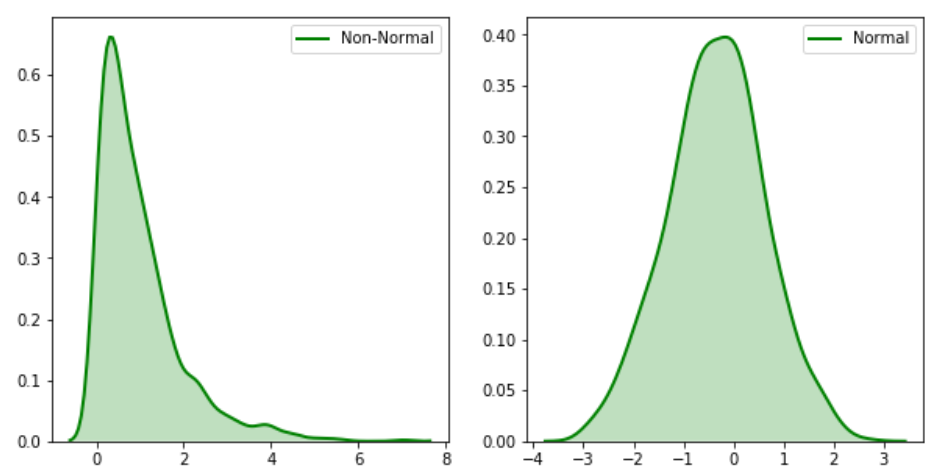
\includegraphics[width=0.5\textwidth]{output275.png}
        \hfill
        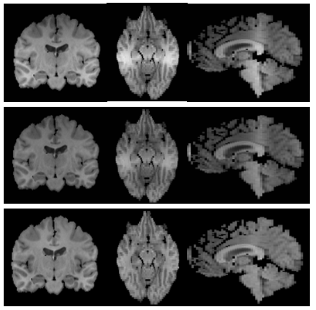
\includegraphics[width=0.4\textwidth]{brains.png}
    \end{figure}
\end{frame}


\begin{frame}{Contenidos}
  \tableofcontents
  % possibilité d'ajouter l'option [pausesections]
\end{frame}
\section{Coeficientes de Correlación}
\subsection{Coeficiente de Información Máxima}
\begin{frame}
    \begin{center}
        {\LARGE\bf 1.- Coeficientes de Correlación}
        \pause

        {\Large  Coeficiente de Información Máxima (MIC)}
    \end{center}
\end{frame}




\begin{frame}{Coeficientes de Correlación: MIC}
    \begin{itemize}
        \item Propuesto por Reshef en 2011 en "Detecting Novel Associations in Large Data Sets".
        \pause
        \item Se basa en la idea de que, si hay una relación fuerte entre dos variables, una podría ser predecida en base a la otra.
        \pause
        \item Permite detectar relaciones débiles pero importantes.
    \end{itemize}
    \pause
    \begin{block}{Información mutua}
    Dada una distribución bivariada $P(x,y)$, definimos:
        \begin{equation*}
            \mathrm{I}(X ; Y)=\int_{\mathcal{Y}} \int_{\mathcal{X}} P_{(X, Y)}(x, y) \log \left(\frac{P_{(X, Y)}(x, y)}{P_{X}(x) P_{Y}(y)}\right)dxdy
        \end{equation*}
    \end{block}
\end{frame}

\begin{frame}{Coeficientes de Correlación: MIC}
    Sea D un conjunto finito de pares ordenados, podemos particionar el espacio malla $G$ de resolución $x \times y$.
    \begin{figure}[H]
        \centering
        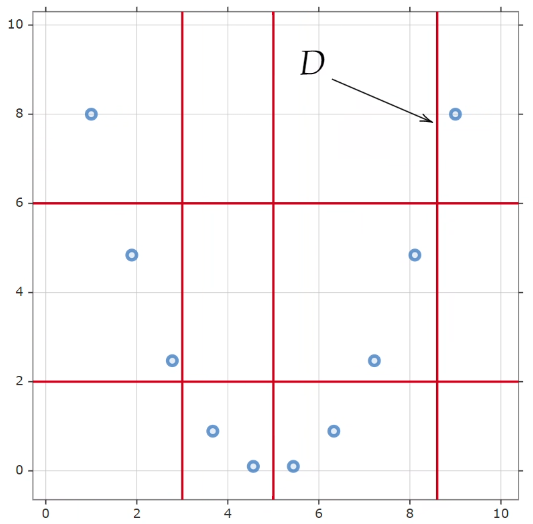
\includegraphics[width=0.3\textwidth]{mallaG4x3.png}
    \end{figure}
    \pause
    \begin{block}{Distribución inducida por una malla}
        Dado una malla $G$, llamaremos $D|_G$ la distribuci\'on inducida por los puntos de $D$ en las celdas de $G$, i.e., la distribuci\'on en las celdas de $G$ obtenida al dejar que la funci\'on de densidad de probabilidad en cada celda sea la fracci\'on de puntos de $D$ que caen en esa celda.
    \end{block}
    
\end{frame}

\begin{frame}{Coeficientes de Correlación: MIC}
    \begin{figure}[H]
        \centering
        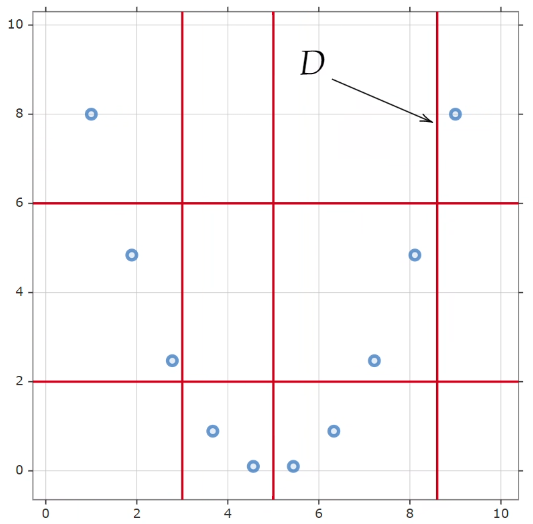
\includegraphics[width=0.3\textwidth]{mallaG4x3.png}
    \end{figure}
    \pause
    \begin{block}{Densidad}
        Para la malla definica en la figura, definimos la función de densidad como:
        \begin{equation*}
            f_{D|_G}(i,j) = \left\{\begin{array}{lr}
                \frac{1}{10} & \text{si } (i,j) \in \{ (1,3), (4,1)\} \\
                \frac{2}{10}, & \text{si }(i,j) \in \{ (1,2), (2,1), (3,1),(3,2)\}  \\
                0, & \text{Otro caso.}
                \end{array}\right.
        \end{equation*}
    \end{block}
\end{frame}


\begin{frame}{Coeficientes de Correlación: MIC}
    \begin{block}{Máximo sobre todas las mallas}
        Para un conjunto finito $D\in\mathcal{R}  ^2$ y enteros positivos $x,y$, definimos:
        $$
        I^*(D,x,y)=\max I(D|_G)
        $$
    \end{block}
    \pause
    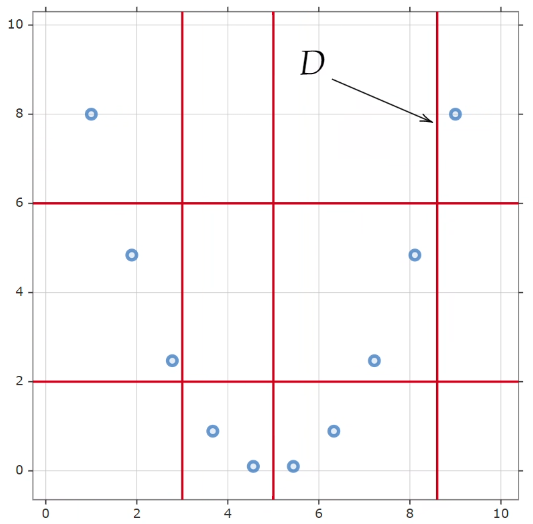
\includegraphics[width=0.4\textwidth]{mallaG4x3.png}
    \hfill
    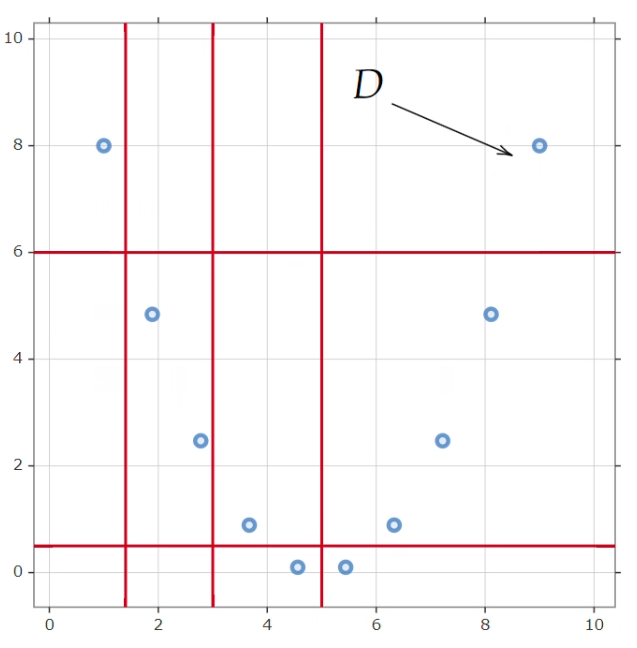
\includegraphics[width=0.4\textwidth]{mallaG4x3_2.png}
\end{frame}

\begin{frame}{Coeficientes de Correlación: MIC}
    \begin{block}{Máximo sobre todas las mallas}
        Para un conjunto finito $D\in\mathcal{R}  ^2$ y enteros positivos $x,y$, definimos:
        $$
        I^*(D,x,y)=\max I(D|_G)
        $$
    \end{block}
    \begin{block}{Matriz Característica}
        Definimos la siguiente matriz       
        \begin{equation*}
	    	M(D)_{x, y}=\frac{I^{*}(D, x, y)}{\log \min \{x, y\}}
        \end{equation*}
    \end{block}
\end{frame}

\begin{frame}{Coeficientes de Correlación: MIC}
     
    \begin{block}{Coeficiente de Información Máxima}
        Definido por Reshef en 2011. Dado un conjunto de datos bivariado, tenemos:
        \begin{equation*}
	    	\operatorname{MIC}(D)=\max _{x y<B(n)}\left\{M(D)_{x, y}\right\}
        \end{equation*}
        donde $\omega(1)<B(n) \leq O\left(n^{1-\varepsilon}\right)$ para alg\'un $0<\varepsilon<1$. En el artículo utilizan $B(n)=n^{0.6}$.
    \end{block}
\end{frame}


\begin{frame}{Coeficientes de Correlación: MIC}
    ¿Cómo calculamos el MIC en la práctica?
    \pause

    Utilizamos $MIC_{e}$, para estimar $MIC_*$, que el valor poblacional de MIC.
    \pause 
    Para esto usamos la matriz equicaracteristica.
    
    \begin{figure}
        \centering
        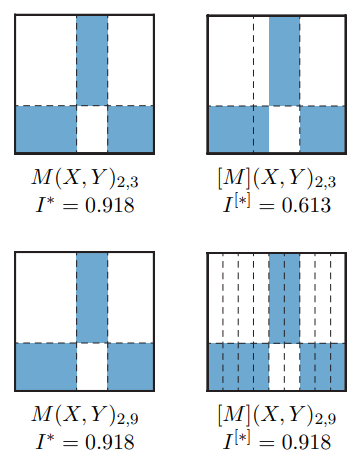
\includegraphics[width=0.4\textwidth]{figuras/figure_1_reshef_2016.png}
    \end{figure}
\end{frame}

\begin{frame}{Coeficientes de Correlación: MIC}
    ¿Cómo calculamos el MIC en la práctica?


    Utilizamos $MIC_{e}$, para estimar $MIC_*$, que es el valor poblacional de MIC.

    \begin{figure}
        \centering
        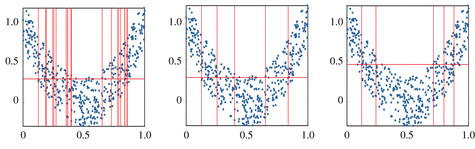
\includegraphics[width=0.4\textwidth]{rsos201424f03.png}
    \end{figure}
    \pause
    Propuesto por Reshef et al (2016) "Measuring Dependence Powerfully and Equitably"
\end{frame}


\subsection{Correlaci\'on y Covarianza por Distancia}
\begin{frame}
    \begin{center}
        {\LARGE\bf 1.-  Coeficientes de Correlación}
        \pause

        {\Large  Correlaci\'on y Covarianza por Distancia (dCor)}
    \end{center}
\end{frame}

\begin{frame}{Coeficientes de Correlación: dCor}
     Propuesto por Székely et al. (2007) en  "\textit{Measuring and testing independence by correlation of distances}". Este se plantea como una generalizaci\'on de la correlaci\'on de Pearson, en particular cumple:
    \pause
    \begin{enumerate}
        \item $\mathcal{R}(X,Y)$ est\'a definido para $X,Y$ de dimensi\'on aleatoria.
        \pause
        \item $\mathcal{R}(X,Y) = 0$ caracteriza la independencia de $X$ e $Y$.
    \end{enumerate}
    \pause
    Busca encontrar relaciones no lineales entre dos conjuntos de datos.
    \pause
    \begin{block}{Covarianza por Distancia}
        La Covarianza por distancia (dCov) entre los vectores aleatorios $X$ e $Y$ con primeros momentos finitos es el n\'umero no negativo $\mathcal{V}(X, Y)$ definido por:
        \begin{equation*}
            \begin{aligned}\label{dcov_formula}
                \mathcal{V}^2(X, Y) & =\left\|f_{X, Y}(t, s)-f_X(t) f_Y(s)\right\|^2 \\
                & =\frac{1}{c_p c_q} \int_{\mathcal{R}^{p+q}} \frac{\left|f_{X, Y}(t, s)-f_X(t) f_Y(s)\right|^2}{|t|_p^{1+p}|s|_q^{1+q}} d t d s .
                \end{aligned}
        \end{equation*}
    \end{block}
\end{frame}


\begin{frame}{Coeficientes de Correlación: dCor}
    \begin{block}{Varianza por distancia}
        Se define como:

        $$
        \mathcal{V}^2(X)=\mathcal{V}^2(X, X)=\left\|f_{X, X}(t, s)-f_X(t) f_X(s)\right\|^2 .
        $$
        
    \end{block}
    \pause
    Por definici\'on de la norma $\|\cdot\|$, es claro que  $\mathcal{V}(X, Y) \geq 0$ y $\mathcal{V}(X, Y)=0$ si y solo si $X$ e $Y$ son indepentes.
    \pause
    \begin{block}{Correlaci\'on por Distancia}
        La correlaci\'on por distancia (dCor) entre los vectores aleatorios $X$ e $Y$ con primer momento finito es el n\'unero no negtivo $\mathcal{R}(X, Y)$ definido por:
		$$
		\mathcal{R}^2(X, Y)= \begin{cases}\frac{\mathcal{V}^2(X, Y)}{\sqrt{\mathcal{V}^2(X) \mathcal{V}^2(Y)}}, & \mathcal{V}^2(X) \mathcal{V}^2(Y)>0 \\ 0, & \mathcal{V}^2(X) \mathcal{V}^2(Y)=0\end{cases}.
		$$
    \end{block}
\end{frame}

\begin{frame}{Coeficientes de Correlación: dCor}
    ¿Cómo calculamos dCor en la práctica?
    \pause

    Para vectores $\mathbf{X} = x_1, x_2, \dots, x_p$ e $\mathbf{Y} = y_1, y_2, \dots, y_n$, definimos $\left(a_{k l}\right)=\left(\left|x_k-x_l\right|_nx\right)$ y $\left(b_{k l}\right)=\left(\left|y_k-y_l\right|_q\right)$. Definimos:
    \pause
	$$
	A_{k l}=a_{k l}-\bar{a}_{k .}-\bar{a}_{. l}+\bar{a}_{. .}, \quad k, l=1, \ldots, n,
	$$
	donde
	$$
	\bar{a}_{k .}=\frac{1}{n} \sum_{l=1}^n a_{k l}, \quad \bar{a}_{. l},=\frac{1}{n} \sum_{k=1}^n a_{k l}, \quad \bar{a}_{. .}=\frac{1}{n^2} \sum_{k, l=1}^n a_{k l} .
	$$
	\pause
	De forma analoga, definimos $B_{k l}=b_{k l}-\bar{b}_{k .}-\bar{b}_{\cdot l}+\bar{b}_{. .}$, para $k, l=1, \ldots, n$.
\end{frame}

\begin{frame}{Coeficientes de Correlación: dCor}
    \begin{block}{Correlaci\'on por Distancia muestral}
        La no negativa Covarianza por distancia muestral $\mathcal{V}_n(\mathbf{X}, \mathbf{Y})$ y la Correlaci\'on por distancia muestral $\mathcal{R}_n(\mathbf{X}, \mathbf{Y})$ están definidas por:
        $$
        \mathcal{V}_n^2(\mathbf{X}, \mathbf{Y})=\frac{1}{n^2} \sum_{k, l=1}^n A_{k l} B_{k l},
        $$
        y
        $$
        \mathcal{R}_n^2(\mathbf{X}, \mathbf{Y})= \begin{cases}\frac{\mathcal{V}_n^2(\mathbf{X}, \mathbf{Y})}{\sqrt{\mathcal{V}_n^2(\mathbf{X}) \mathcal{V}_n^2(\mathbf{Y})}}, & \mathcal{V}_n^2(\mathbf{X}) \mathcal{V}_n^2(\mathbf{Y})>0 \\ 0, & \mathcal{V}_n^2(\mathbf{X}) \mathcal{V}_n^2(\mathbf{Y})=0\end{cases},
        $$
        respectivamente. Adem\'as la Varianza por distancia muestral $\mathcal{V}_n(\mathbf{X})$ est\'a definida por
        $$
        \mathcal{V}_n^2(\mathbf{X})=\mathcal{V}_n^2(\mathbf{X}, \mathbf{X})=\frac{1}{n^2} \sum_{k, l=1}^n A_{k l}^2 .
        $$
    \end{block}
\end{frame}

\begin{frame}{Coeficientes de Correlación}
    En resumen, 
    \pause
    \begin{block}{MIC}
        El coeficiente de información máxima (MIC) se basa en la idea de que, si hay una relación fuerte entre dos variables, una podría ser predecida en base a la otra. Permite detectar relaciones débiles pero importantes.
    \end{block}
    \pause
    \begin{block}{dCor}
        La Correlación por Distancia (dCor) es una generalización de la correlación de Pearson que busca encontrar relaciones no lineales entre dos variables, en particular establecer una forma de caracterizar independencía entre dos distribuciónes.
    \end{block}
\end{frame}



\section{Análisis y Procesamiento de Imágenes}
\begin{frame}
    \begin{center}
        {\LARGE\bf Análisis y Procesamiento de Imágenes}
    \end{center}
\end{frame}

\begin{frame}{Análisis y Procesamiento de Imágenes}
    ¿Qué es una imagen?
    \pause
    \begin{center}
        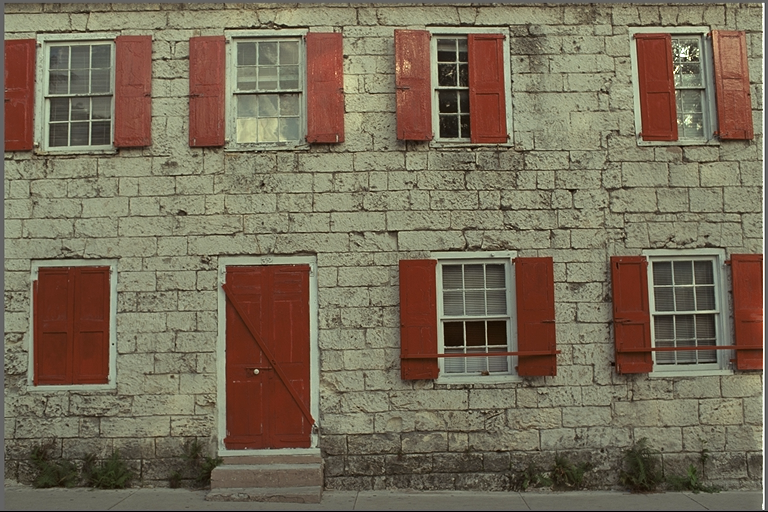
\includegraphics[width=0.8\textwidth]{1.png}
    \end{center}
    \pause
    Una representación visual de un objeto.
\end{frame}

\begin{frame}{Análisis y Procesamiento de Imágenes}
    \begin{block}{Representación de una Imagen}
        Una imagen es una representaci\'on visual de un objeto, y se puede definir como una funci\'on bidimensional $f(x,y)$, como se muestra en la siguiente ecuaci\'on:

        $$
        f(x, y)=\left[\begin{array}{cccc}
        f(0,0) & f(0,1) & \cdots & f(0, N-1) \\
        f(1,0) & f(1,1) & \cdots & f(1, N-1) \\
        \vdots & \vdots & & \vdots \\
        f(M-1,0) & f(M-1,1) & \cdots & f(M-1, N-1)
        \end{array}\right]
        $$

        Donde $M$ y $N$ son las dimensiones de la imagen.
    \end{block}
\end{frame}

\begin{frame}{Análisis y Procesamiento de Imágenes}
    \begin{figure}[H]
        \centering
        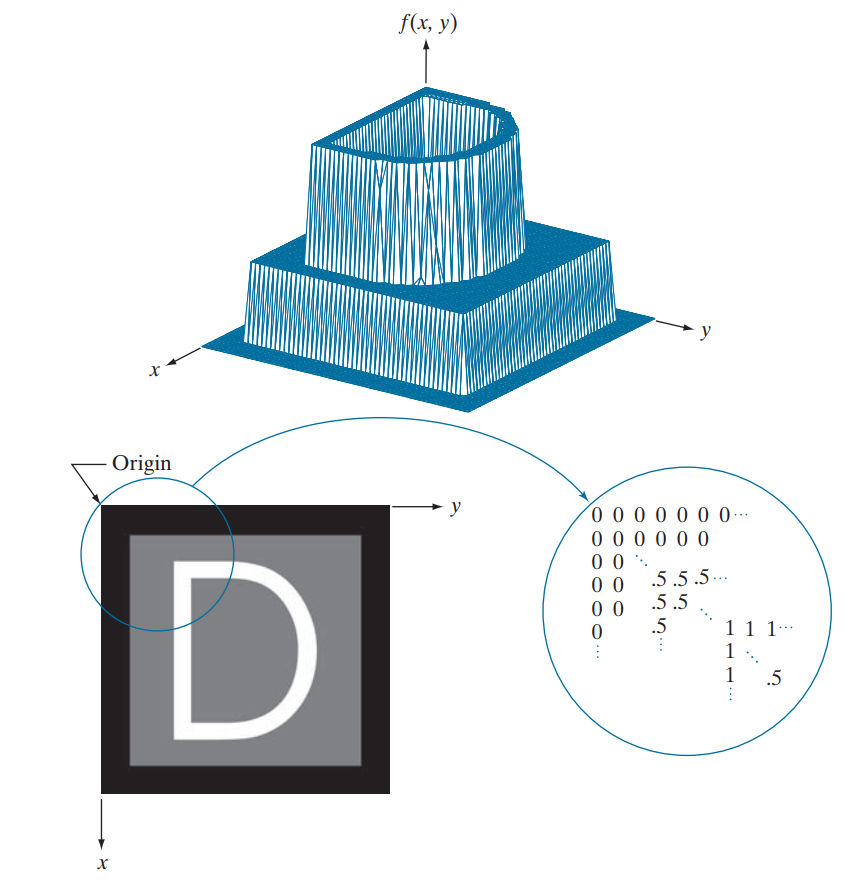
\includegraphics[width=0.5\textwidth]{dip_4_fig2_18.png}
    \end{figure}   
    \pause     
    (a) Como una superficie. 
    \pause 
    (b) Como un conjunto de intensidades visuales. 
    \pause 
    (c) Como un conjunto numérico en 2D. 

\end{frame}

\begin{frame}{Análisis y Procesamiento de Imágenes}
    \begin{figure}[H]
        \centering
        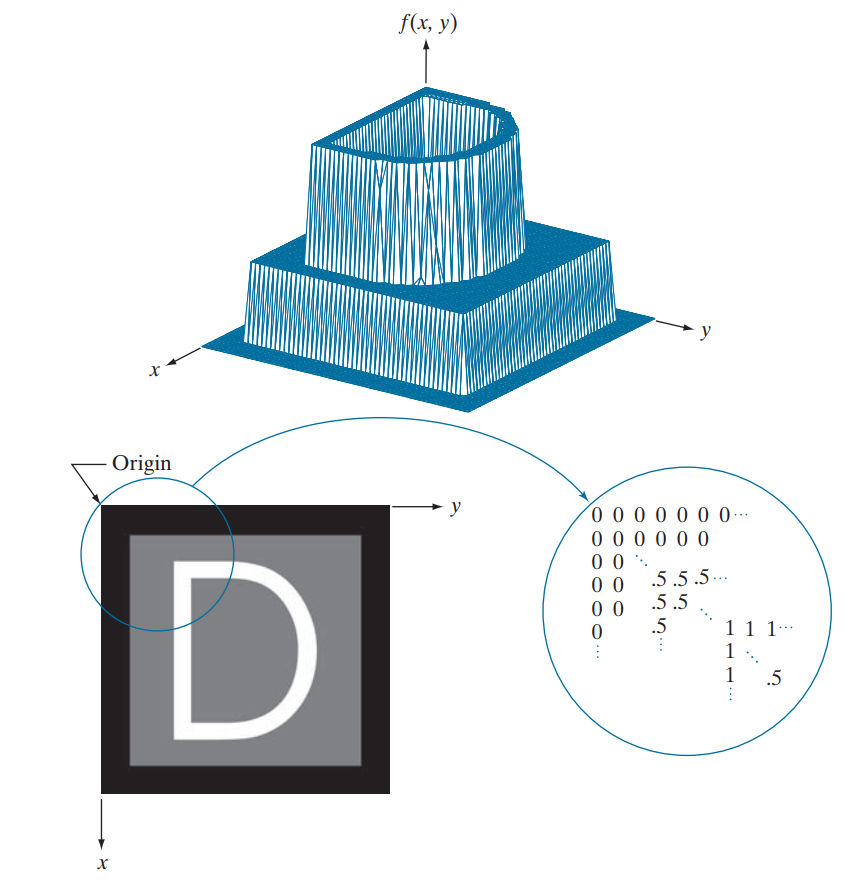
\includegraphics[width=0.5\textwidth]{dip_4_fig2_18.png}
    \end{figure}   


    Notemos que los valores de las intensidades de las imágenes suelen ser valores finitos y discretos. En general es común que estos valores sean números enteros entre $[0, 255]$, o numeros reales entre $[0, 1]$.

\end{frame}

\begin{frame}{Análisis y Procesamiento de Imágenes}
    ¿Qué imágenes usaremos para el análisis? 
    \pause
    \begin{figure}[H]
        \centering
        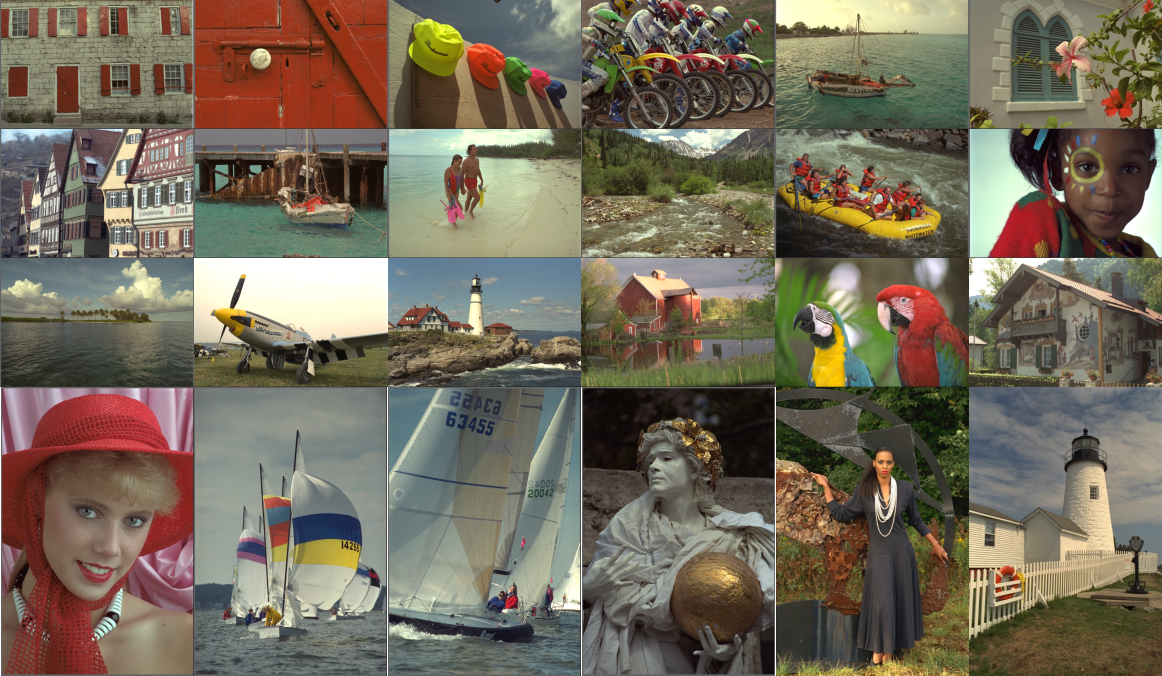
\includegraphics[width=0.8\textwidth]{all_images_grid.png}
    \end{figure}      
    Correponde a \textit {Kodak Lossless True Color Image Suite}, de tamaño $768 \times 512$ pixeles.
\end{frame}

\begin{frame}{Análisis y Procesamiento de Imágenes}
    Las imágenes a color corresponden, en general, a tres canales de color: Rojo (R), Verde (G), y Azul (B). Cada uno con su respectiva matriz.
    \pause
    \begin{figure}[H]
        \centering
        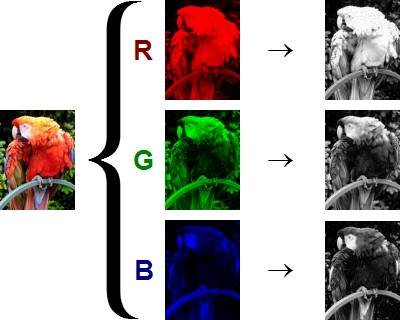
\includegraphics[width=0.55\textwidth]{RGB_channels_separation.png}
    \end{figure} 
    \pause
    Necesitamos convertir las imágenes a escala de grises para el análisis.
\end{frame}

\begin{frame}{Análisis y Procesamiento de Imágenes}
    \begin{block}{Im\'agenes Escala de Grises}
        Nos interesa trabajar con escala de grises, lo hacemos de la siguiente forma.

        \begin{equation*}
            I(x, y)=0.299 R(x, y)+0.687 G(x, y)+0.114 B(x, y), 
            \label{eq:grayscale}
        \end{equation*}

        que corresponde el canal gris del espacio de colores $YC_bC_r$. A esta candidad le llamaremos Intensidad.
    \end{block}
    \pause
    \begin{figure}[H]
        \centering
        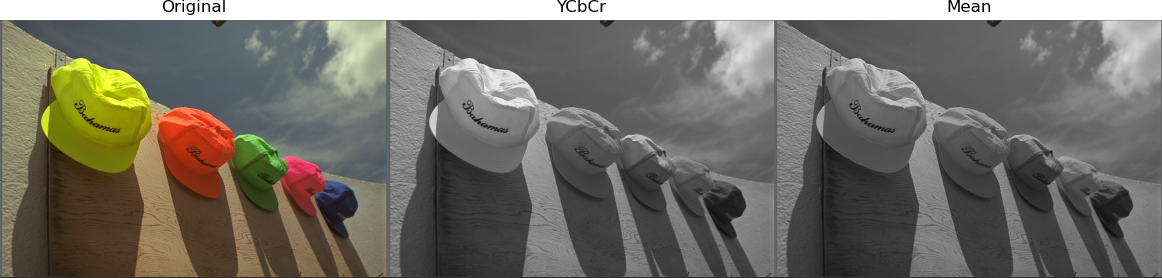
\includegraphics[width=0.8\textwidth]{img_ex_bw.png}
        \caption{Imagen RGB,escala de grises, y promedio simple.}
    \end{figure}
\end{frame}

\begin{frame}{Análisis y Procesamiento de Imágenes}
    \begin{figure}[H]
        \centering
        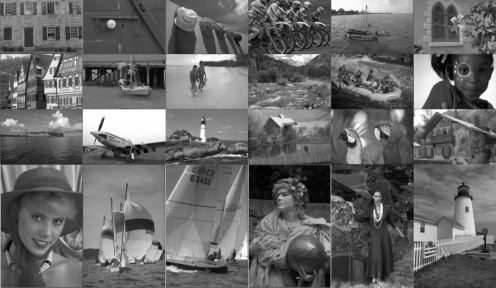
\includegraphics[width=\textwidth]{all_images_grid_bw.png}
    \end{figure}     
\end{frame}

\begin{frame}{Análisis y Procesamiento de Imágenes}
    \begin{center}
        {\Large ¿Cómo comparamos dos imágenes usando MIC o dCor?}
    \end{center}
\end{frame}

\begin{frame}{Análisis y Procesamiento de Imágenes}
    Los métodos de correlación definidos anteriormente están pensados para ser aplicados sobre dos vectores, pero en el caso de imágenes, tenemos una matriz de datos. 
    \pause
    Por lo tanto, necesitamos una forma de transformar una imagen en un vector unidimensional.
    \pause
    \begin{block}{Imagen a Vector}
        Dada una imagen $I(x, y)$, la transformamos a un vector unidimensional  $\hat{I}(t)$, notemos que para este contexto el orden no es relevante. Comparamos estos dos vectores.
    \end{block}
    \pause
    \begin{block}{Histograma}
        Generamos un histograma de los valores intensidad de la imagen, con tantos bins como sea necesario. Comparamos estos histogramas.
    \end{block}
\end{frame}

\begin{frame}{Análisis y Procesamiento de Imágenes}
    \begin{figure}[H]
        \centering
        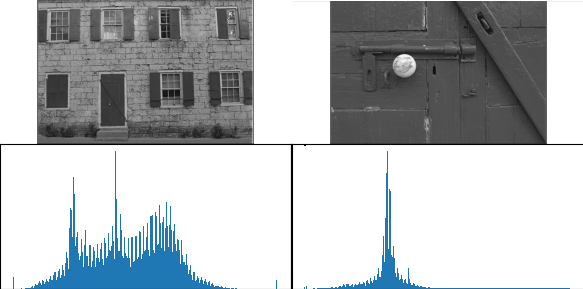
\includegraphics[width=\textwidth]{img_hist.png}
        \caption{Imágenes junto con sus histogramas con ruido.}
    \end{figure}
\end{frame}

\begin{frame}{Análisis y Procesamiento de Imágenes}
    
\includegraphics[width=0.4\textwidth]{Flag_of_France.png}
    \hfill
    
\includegraphics[width=0.4\textwidth]{Flag_of_Russia.png}
\end{frame}

\begin{frame}{Análisis y Procesamiento de Imágenes}
    Dado esto, tenemos tenemos 4 formas de comparar dos imágenes:
    \pause
    \begin{block}{Compración de Imágenes}
        \begin{enumerate}
            \item Comparar los vectores de las imágenes usando MIC.
            \pause
            \item Comparar los vectores de las imágenes usando dCor.
            \pause
            \item Comparar los histogramas de las imágenes usando MIC.
            \pause
            \item Comparar los histogramas de las imágenes usando dCor.
        \end{enumerate}
    \end{block}
    \pause
    Además en los siguientes analisis también se mostrará la correlación de Pearson $\rho$ entre las imágenes, a modo de base de comparación.
\end{frame}

\begin{frame}{Análisis y Procesamiento de Imágenes}
    \begin{center}
        {\Large Ejemplos de comparación de imágenes}
    \end{center}
\end{frame}

\begin{frame}{Análisis y Procesamiento de Imágenes}
    \begin{figure}[H]
        \centering
        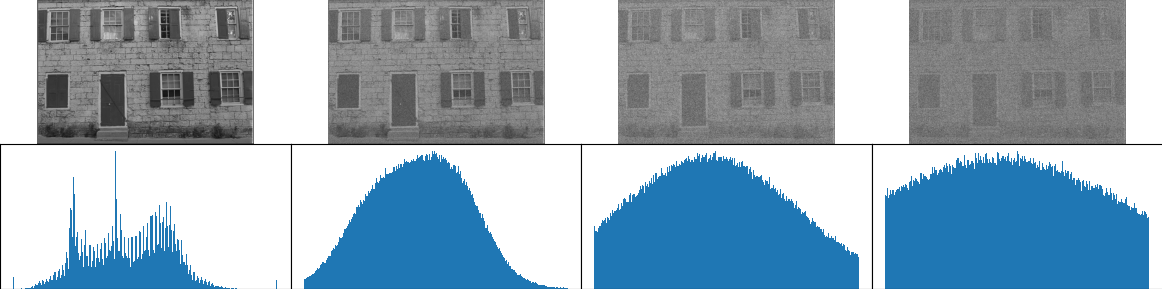
\includegraphics[width=\textwidth]{img_hist_noise_one.png}
    \end{figure}
    Imagen junto con sus histograma con ruido.
\end{frame}
\begin{frame}{Análisis y Procesamiento de Imágenes}
    \begin{figure}[H]
        \centering
        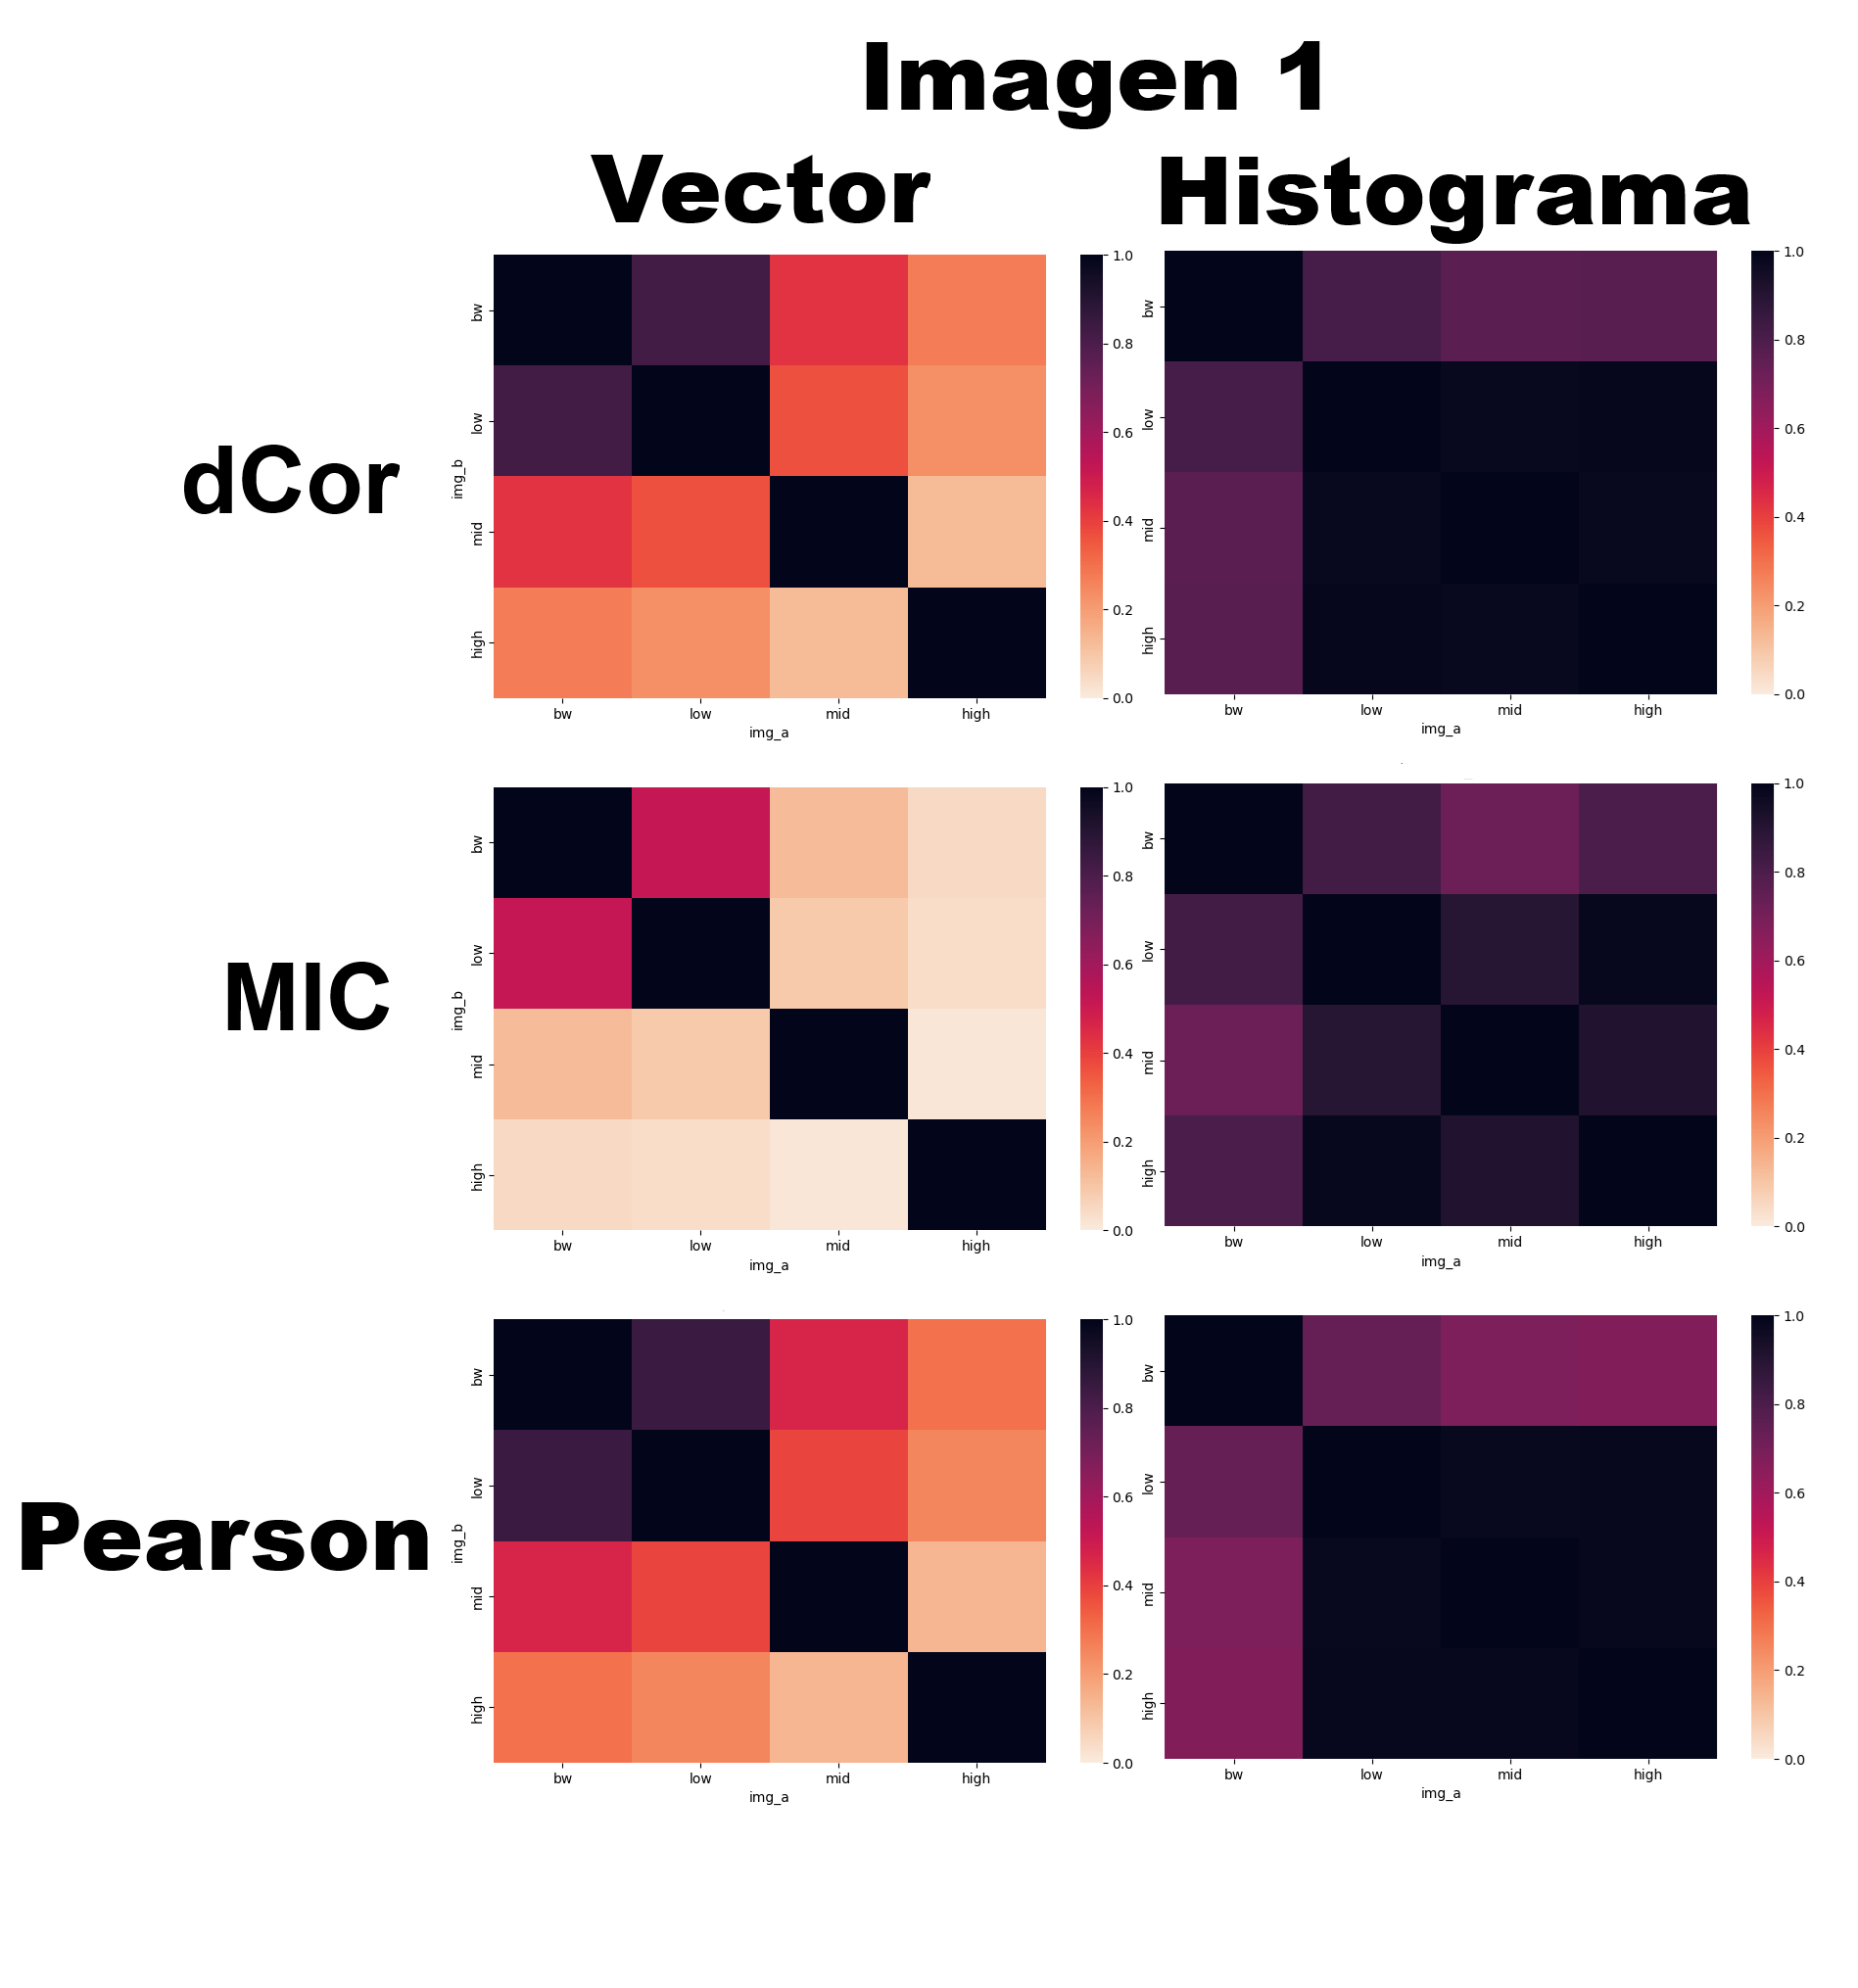
\includegraphics[width=0.4\textwidth]{heatmap_one.png}
    \end{figure}
    Matriz de calor para la imagen 1 del banco, cada mapa de calor corresponde a un m\'etodo de comparaci\'on, ya sea comparando el total de la imagen (izquierda), o el histograma de estas (derecha).
\end{frame}

\begin{frame}{Análisis y Procesamiento de Imágenes}
    \begin{figure}[H]
        \centering
        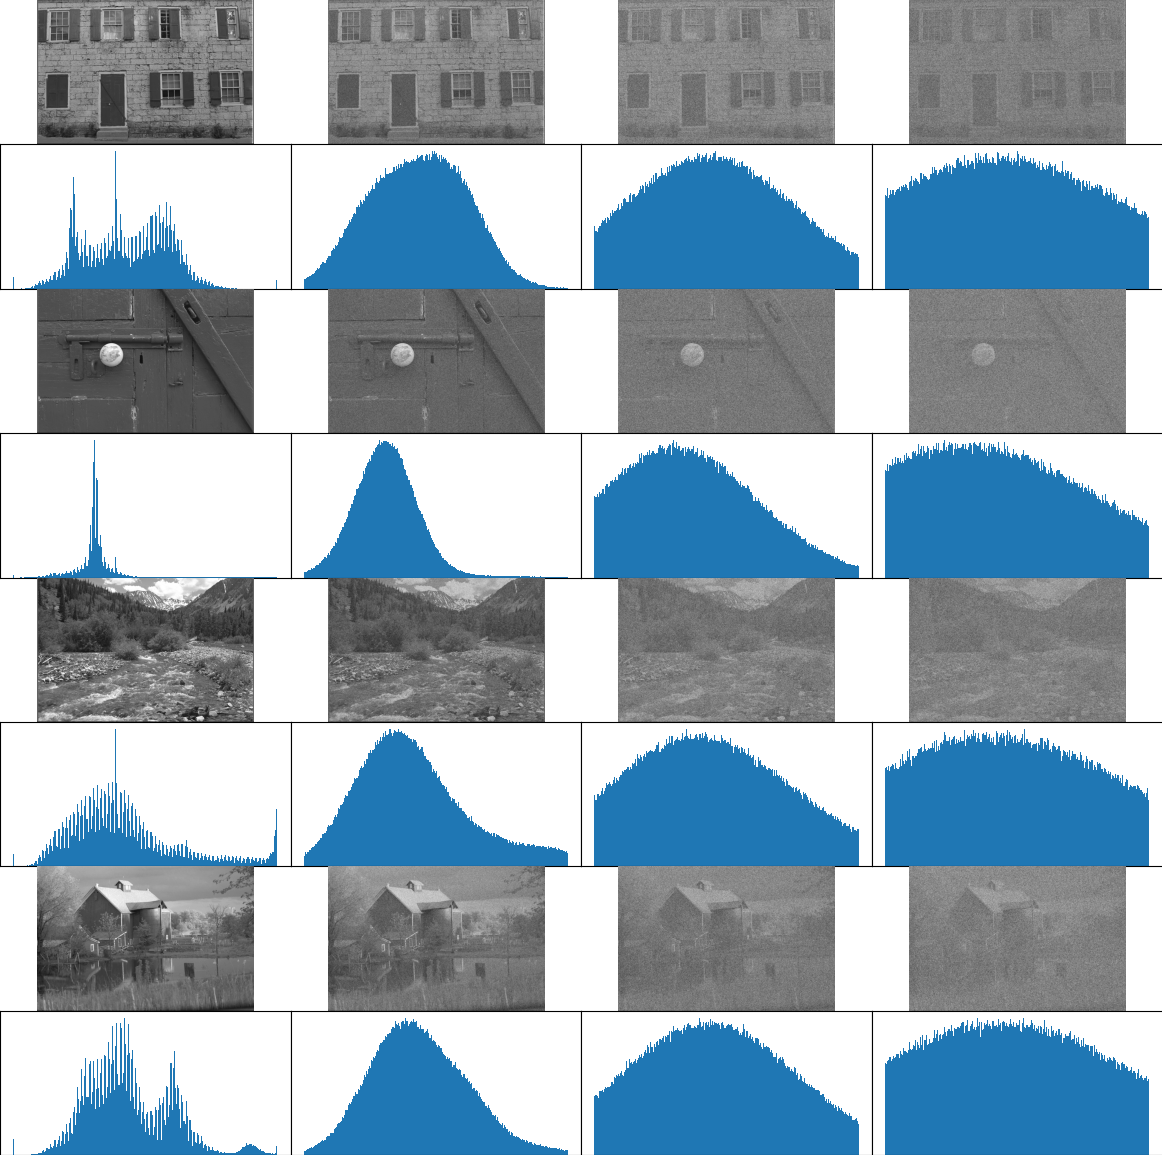
\includegraphics[width=0.6\textwidth]{img_hist_noise.png}
    \end{figure}
    Imágenes junto con sus histogramas con ruido.
\end{frame}

\begin{frame}{Análisis y Procesamiento de Imágenes}
    \begin{figure}[H]
        \centering
        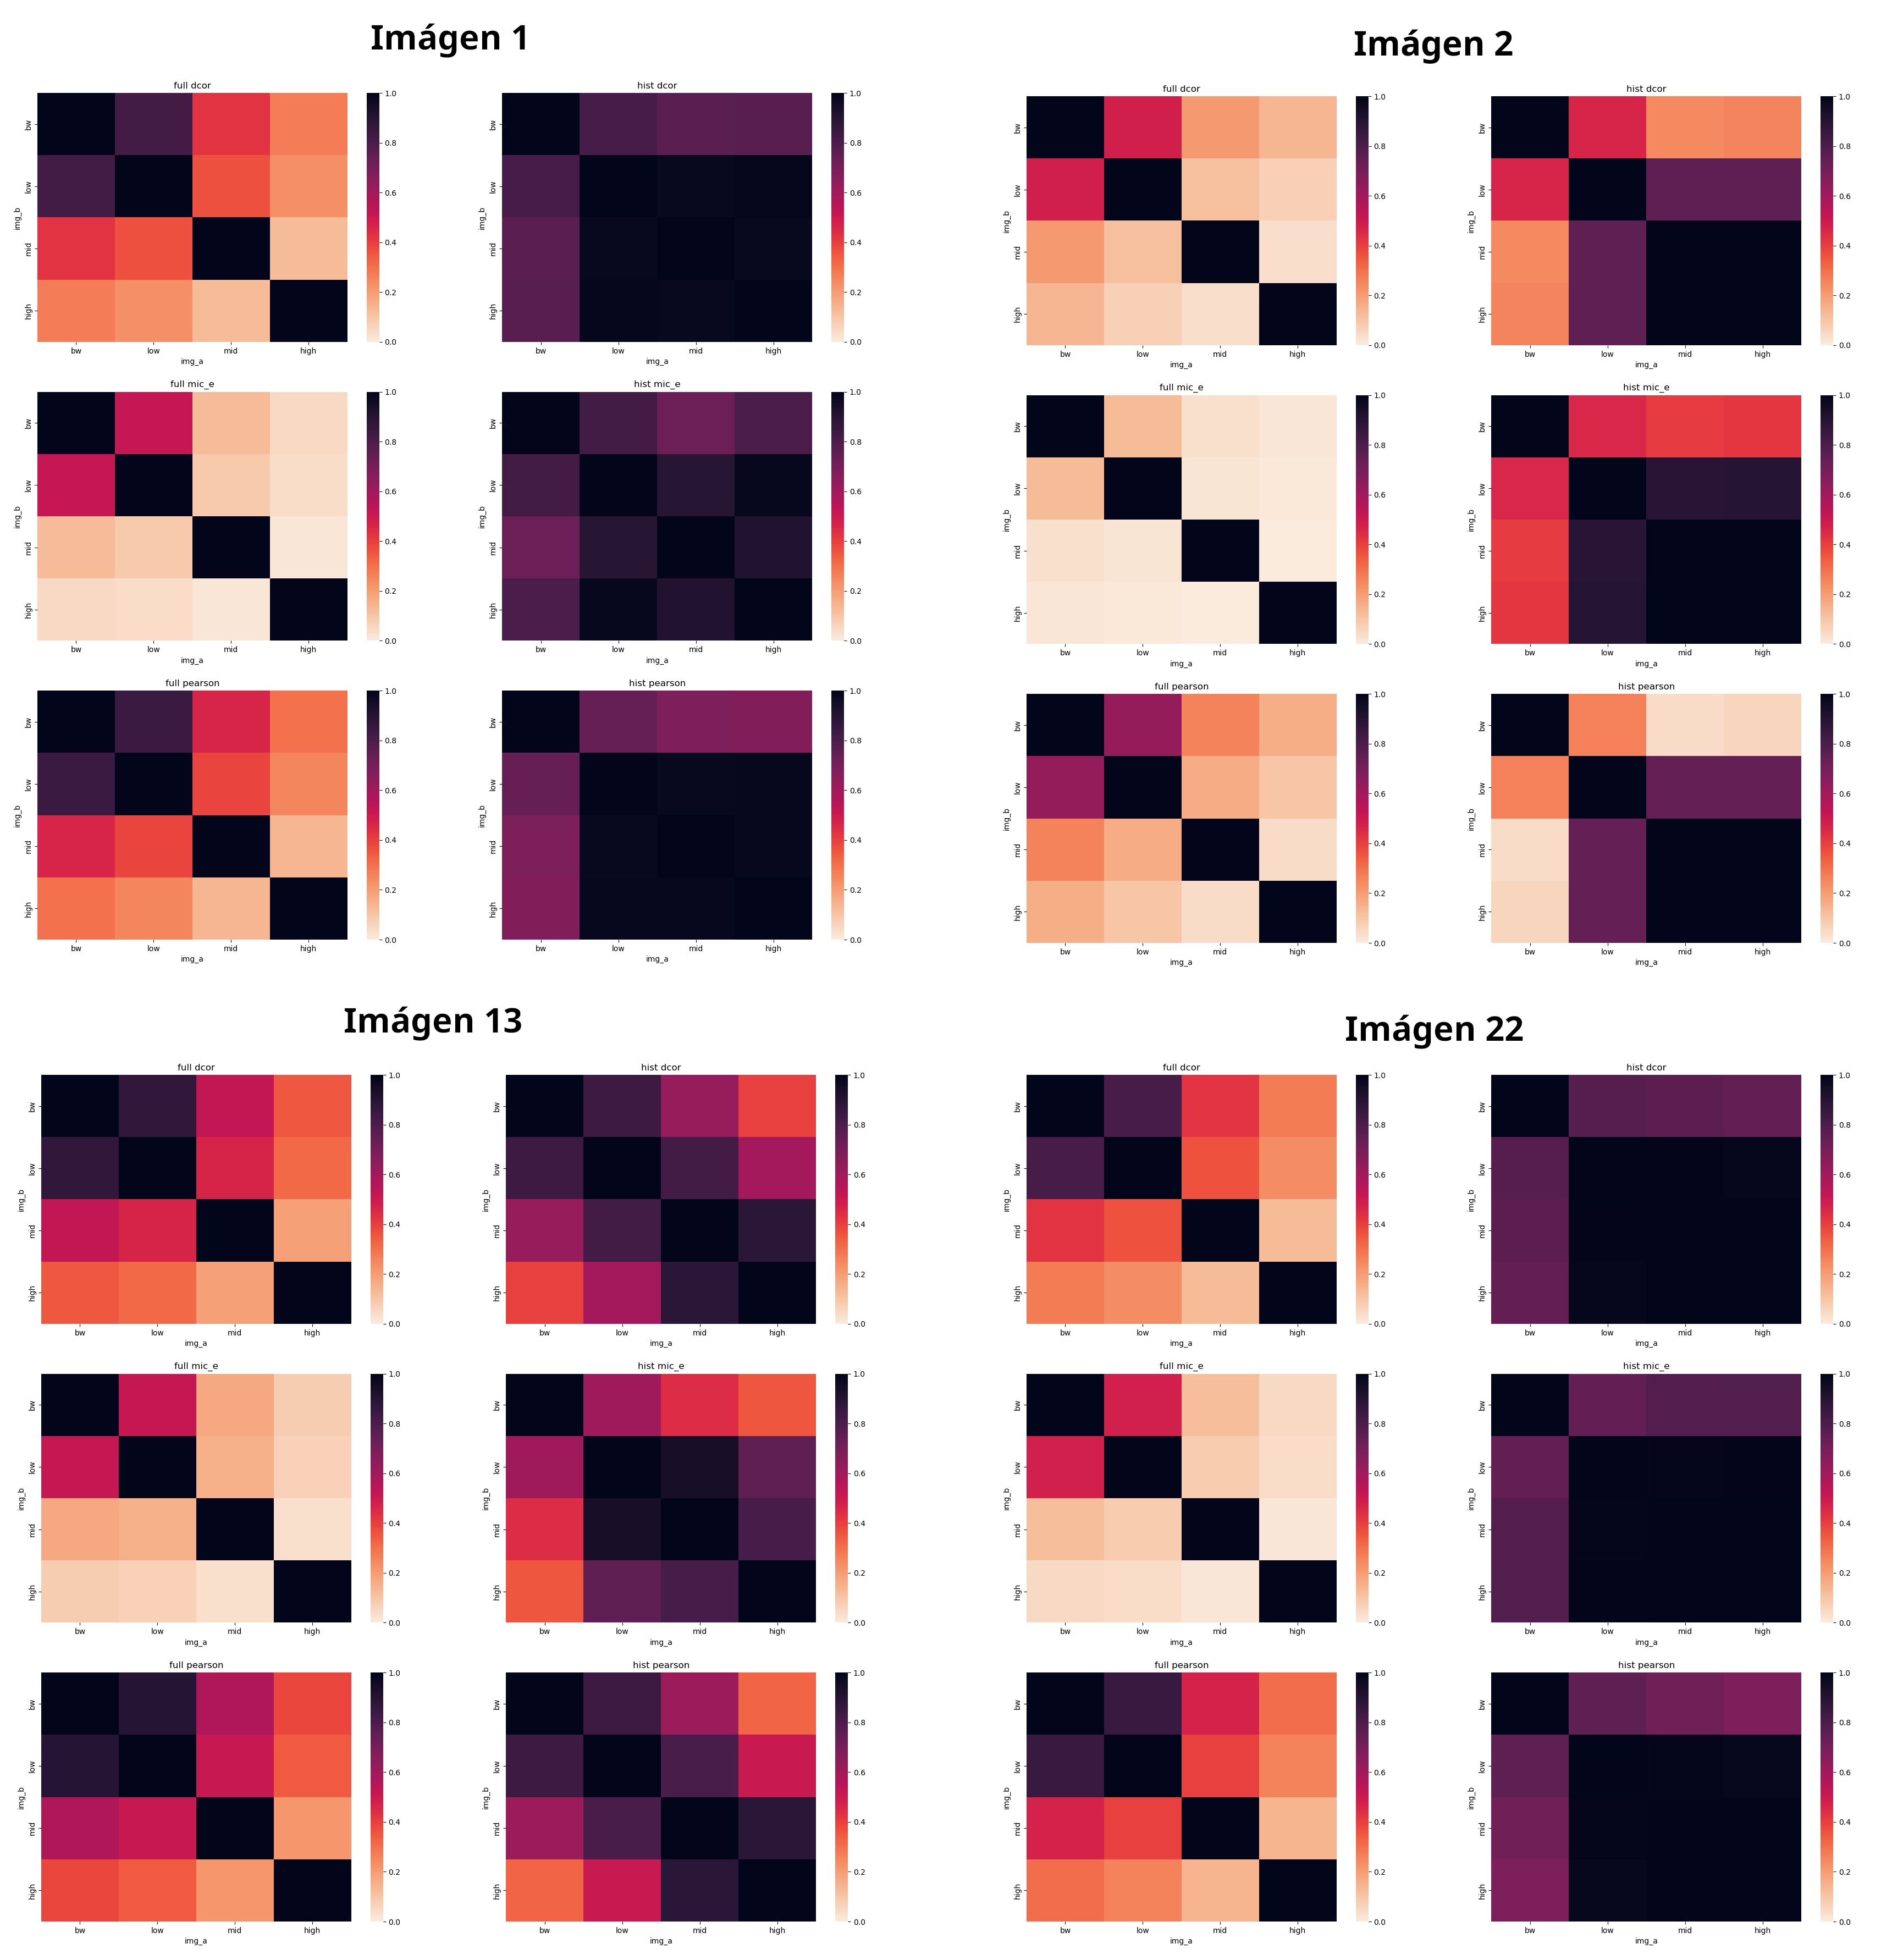
\includegraphics[width=\textwidth]{heatmap_all.png}
    \end{figure}
    Matriz de calor para las imagenes 1, 2, 13, y 22 del banco, cada mapa de calor corresponde a un m\'etodo de comparaci\'on, ya sea comparando el total de la imagen (izquierda), o el histograma de estas (derecha). La cantidad de ruido aumenta de izquierda a derecha, y de arriba hacía abajo.
\end{frame}
\section{La transformación Box-Cox}

\begin{frame}
    \begin{center}
        {\LARGE\bf La transformación Box-Cox}
    \end{center}
\end{frame}



\begin{frame}{La transformación Box-Cox}
    Propuesta por George Box y David Cox en 1964 en su trabajo "\textit{An Analysis of Transformations}", la transformación Box-Cox es una familia de transformaciones que se utilizan para hacer que los datos se asemejen a una distribución normal.
    \pause
    \begin{center}
        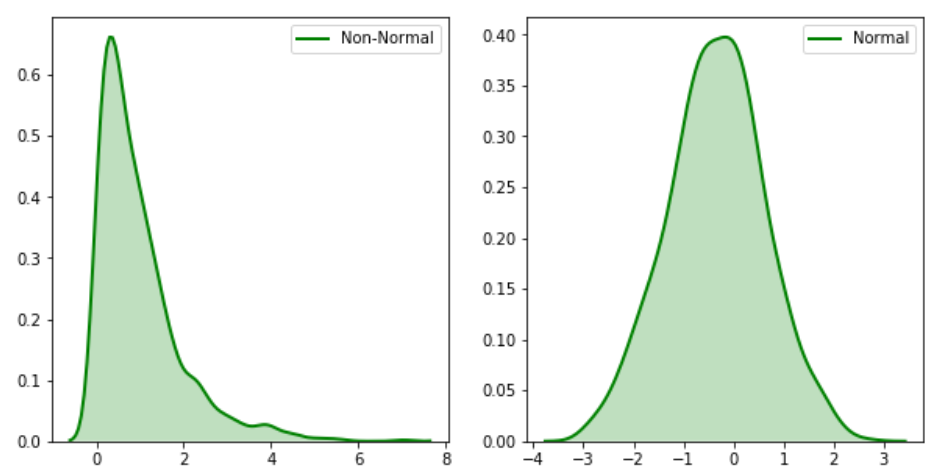
\includegraphics[width=0.4\textwidth]{output275.png}
    \end{center}
    \pause
    \begin{block}{Transformación Box-Cox}
        Dado un vector $Y=(y_1, y_2, ..., y_n)\in\mathcal{R}_{<0}^n$, la transformación Box-Cox se define como:
        \begin{equation*}
            y_i^{(\lambda)}= \begin{cases}\frac{y_i^{\lambda}-1}{\lambda} & (\lambda \neq 0) \\ \log y_i & (\lambda=0)\end{cases}
        \end{equation*}
    \end{block}
\end{frame}

\begin{frame}{La transformación Box-Cox}
    ¿Cómo seleccionamos $\lambda$?

    \pause
    \begin{block}{Verosimilitud}
        \begin{equation*}
            \mathcal{L}(\lambda) \equiv-\frac{n}{2} \log \left[\frac{1}{n} \sum_{j=1}^{n}\left(x_{j}^{\lambda}-\overline{x^{\lambda}}\right)^{2}\right] +(\lambda-1) \sum_{j=1}^{n} \log x_{j}
        \end{equation*}
    \end{block}
    \pause
    La versimilitud es una función que mide la probabilidad de que los datos observados hayan sido generados por un modelo estadístico. En este caso, la versimilitud mide la probabilidad de que los datos observados hayan sido generados por una distribución normal.

    Notemos que en la práctica, el valor de $\lambda$ se selecciona dentro de un rango de valores como $[-5, 5]$, o $[-2, 2]$.
\end{frame}

\begin{frame}{La transformación Box-Cox}

    ¿Cómo aplicamos la transformación Box-Cox a imágenes?
    \pause

    Tenemos una imagen $I(x, y)$, definimos $\mathcal{F}^{\lambda_{\cdot}}(x, y) = I(x, y)^{(\lambda)}$. Como la transformación Box-Cox aplicada a la intensidad del pixel $(x, y)$.
    \pause
    \begin{block}{Box-Cox para imagenes}
        Sea $\mathcal{F}^{\lambda_{\cdot}}(x, y)$ las imagen transformada para alg\'un $\lambda_\cdot$ seleccionado, entonces definimos BCI como:

        \begin{equation*}
            BCI = \frac{\left(\mathcal{F}^{\lambda_{\cdot}}(x, y) - \min\left(\mathcal{F}^{\lambda_{\cdot}}(x, y)\right)\right)}{\left(\max\left(\mathcal{F}^{\lambda_{\cdot}}(x, y)\right) - \min\left(\mathcal{F}^{\lambda_{\cdot}}(x, y)\right)\right)}
        \end{equation*}
    \end{block}
    \pause
    Más adelante discutiremos como seleccionamos $\lambda$ para imágenes. Pero antes veamos algunos ejemplos.
\end{frame}

\begin{frame}{La transformación Box-Cox}
    \begin{center}
        {\Large Ejemplos de BCI}
    \end{center}
\end{frame}

\begin{frame}{La transformación Box-Cox}
    \begin{figure}
        \centering
        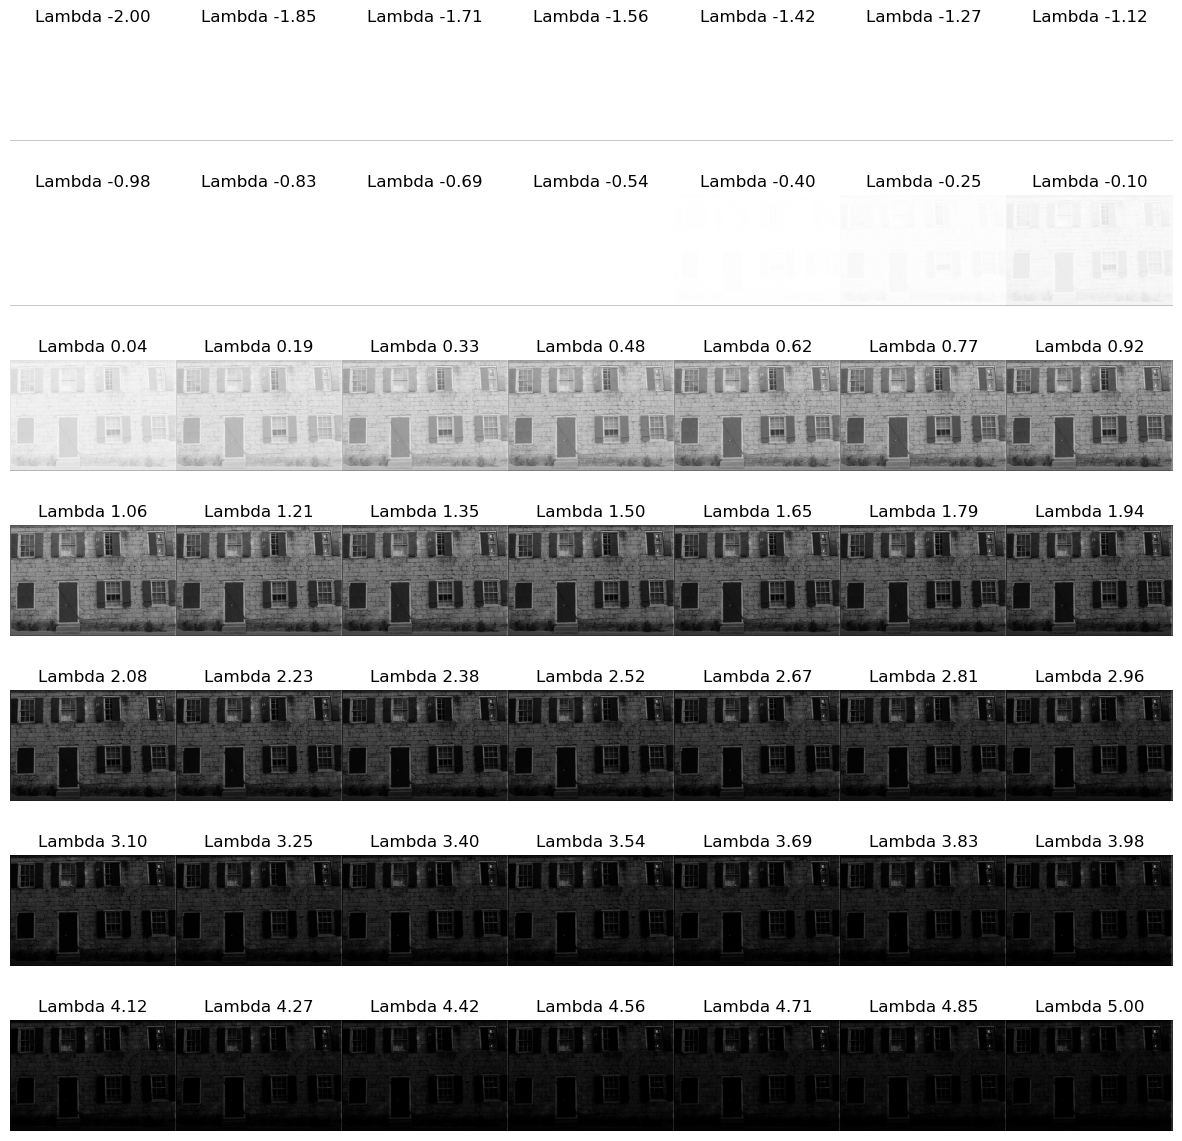
\includegraphics[width=0.6\textwidth]{all_lambda_1.png}
        \caption{Transformaciones de la imagen 1.}
        \label{fig:all_lambda_1}
    \end{figure}
\end{frame}


\begin{frame}{La transformación Box-Cox}
    \begin{figure}
        \centering
        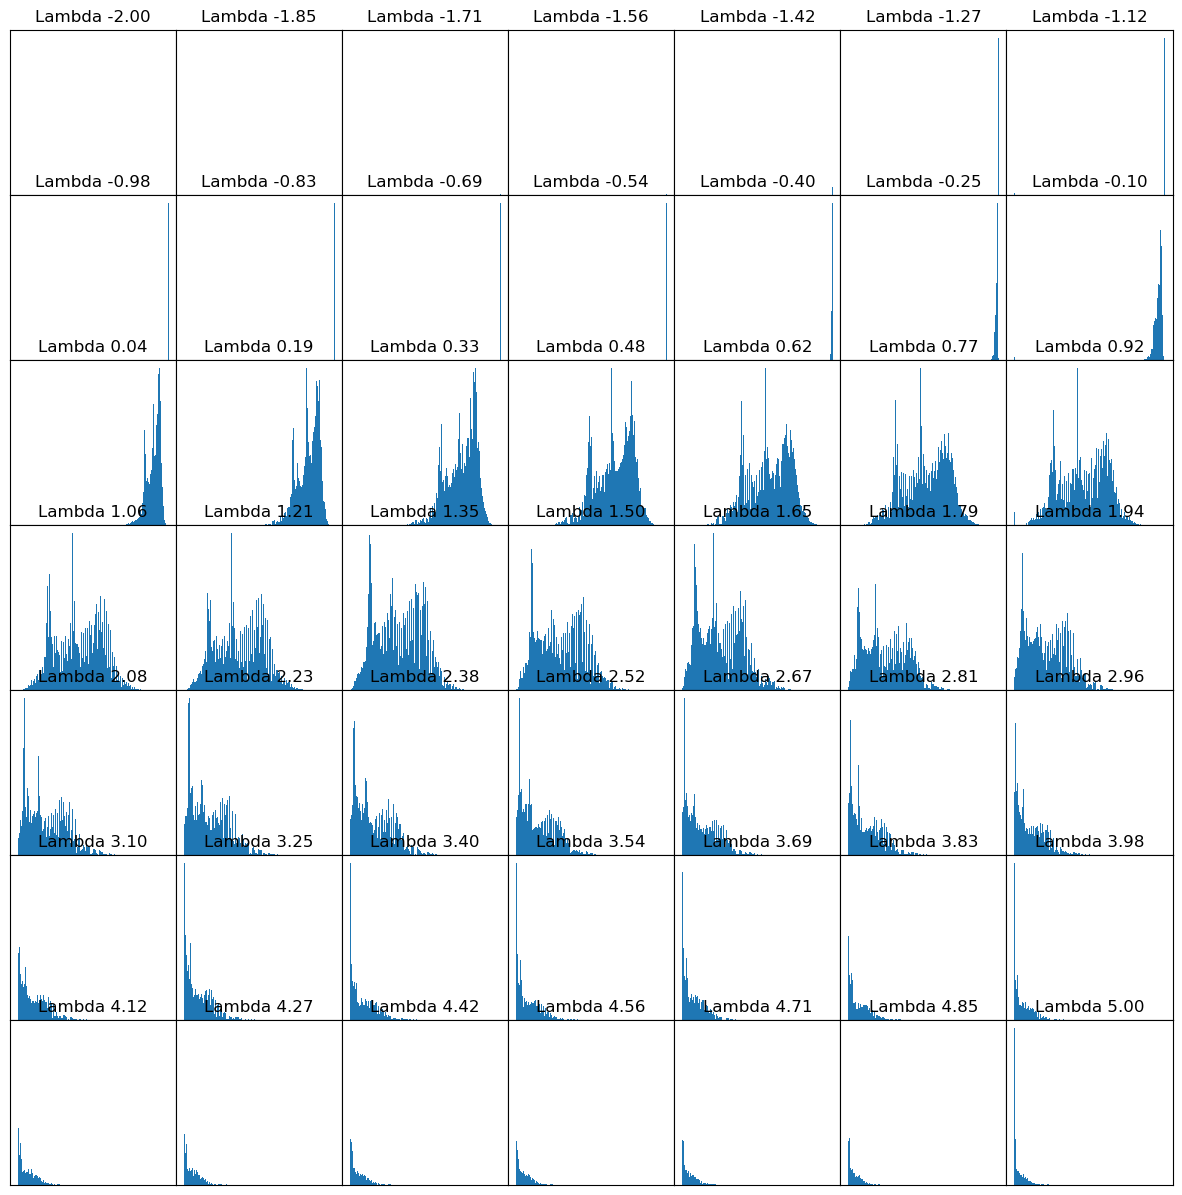
\includegraphics[width=0.6\textwidth]{all_lambda_hist_1.png}
        \caption{Histograma de las transformaciones de la imagen 1.}
        \label{fig:img_bci_hist_1}
    \end{figure}
\end{frame}



\begin{frame}{La transformación Box-Cox}
    \begin{figure}
        \centering
        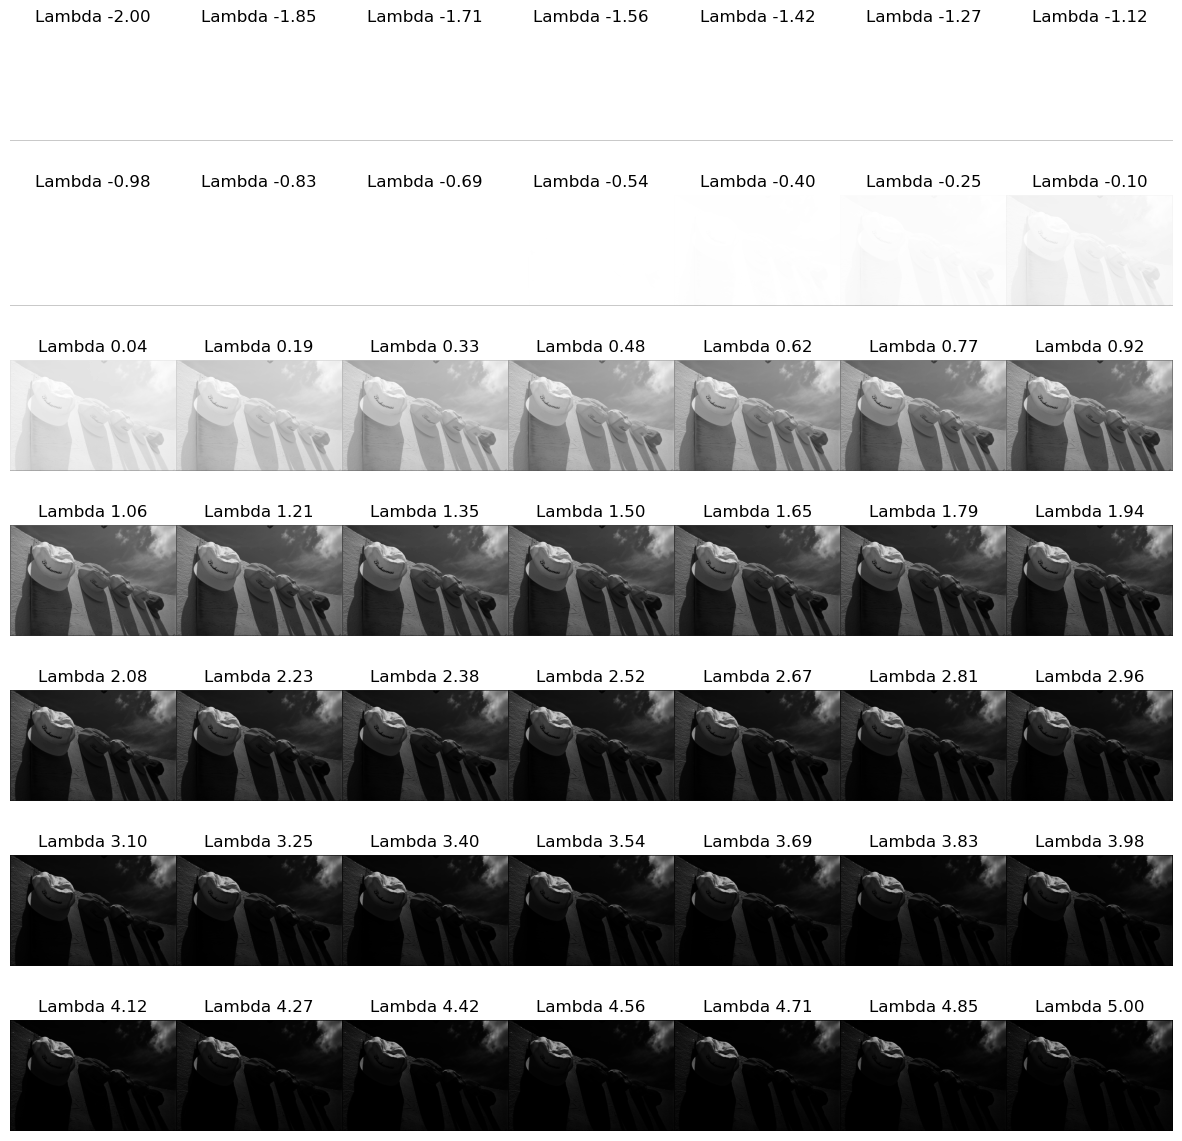
\includegraphics[width=0.6\textwidth]{all_lambda_3.png}
        \caption{Transformaciones de la imagen 3.}
        \label{fig:all_lambda_2}
    \end{figure}
\end{frame}

\begin{frame}{La transformación Box-Cox}
    \begin{figure}
        \centering
        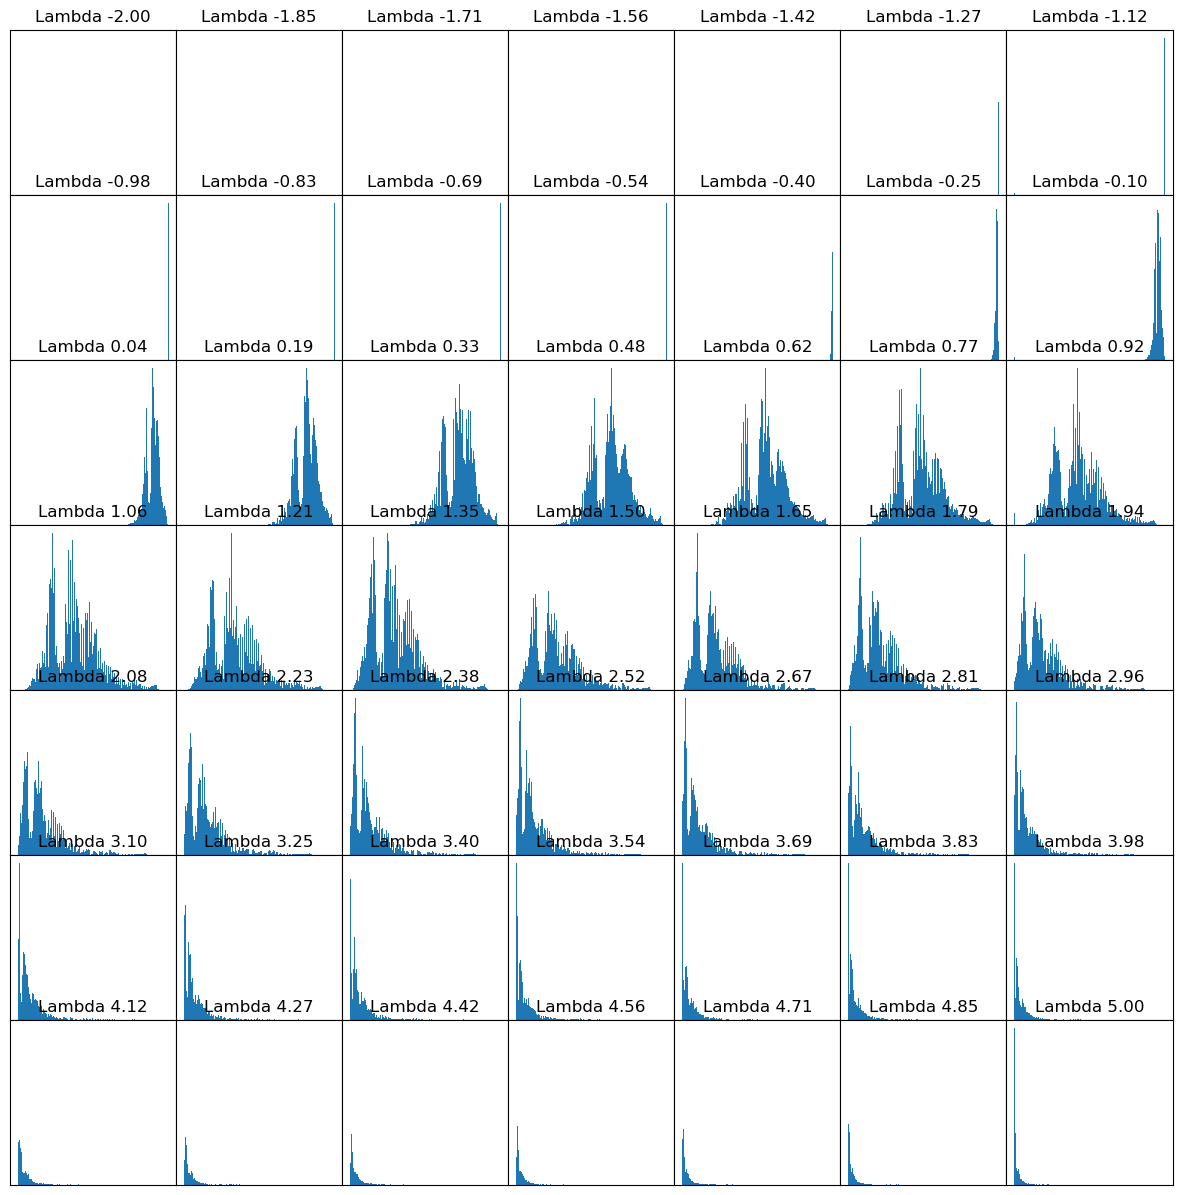
\includegraphics[width=0.6\textwidth]{all_lambda_hist_3.png}
        \caption{Histograma de las transformaciones de la imagen 2.}
        \label{fig:img_bci_hist_2}
    \end{figure}
\end{frame}

\begin{frame}{La transformación Box-Cox}
    \begin{center}
        {\Large ¿Cómo seleccionamos $\lambda$ para imágenes?}
    \end{center}
\end{frame}

\begin{frame}{La transformación Box-Cox}
    \begin{block}{Transformación 1-D}
        Transformar la imagen a un vector unidimensional, usar estos datos para determinar $\lambda$. Propuesto por Lee et al. (2018) en "MR Image Segmentation Using a Power Transformation Approach.". Lo llamamos $\lambda_{full}$.
    \end{block}
    
    \pause
    \begin{block}{Histograma}
        La idea es usar el histograma como un proxy comprimido de de la matriz de datos. Propuesto por Cheddad et al. (2010) en "Transformation for Image Normality and Pattern Classification". Lo llamamos $\lambda_{hist}$.
    \end{block}
    
    \pause
    \begin{block}{Grilla}
        La idea es usar una grilla sobre la imagen para mantener unformacion local al monento de encontrar $\lambda$. Original a la Memoria. Lo llamamos $\lambda_{grid}$.
    \end{block}

\end{frame}

\begin{frame}{La transformación Box-Cox}
    \begin{center}
        {\Large Ejemplos de BCI con $\lambda$'s seleccionados}
    \end{center}
\end{frame}

\begin{frame}{La transformación Box-Cox}
    \begin{figure}[H]
        \centering
        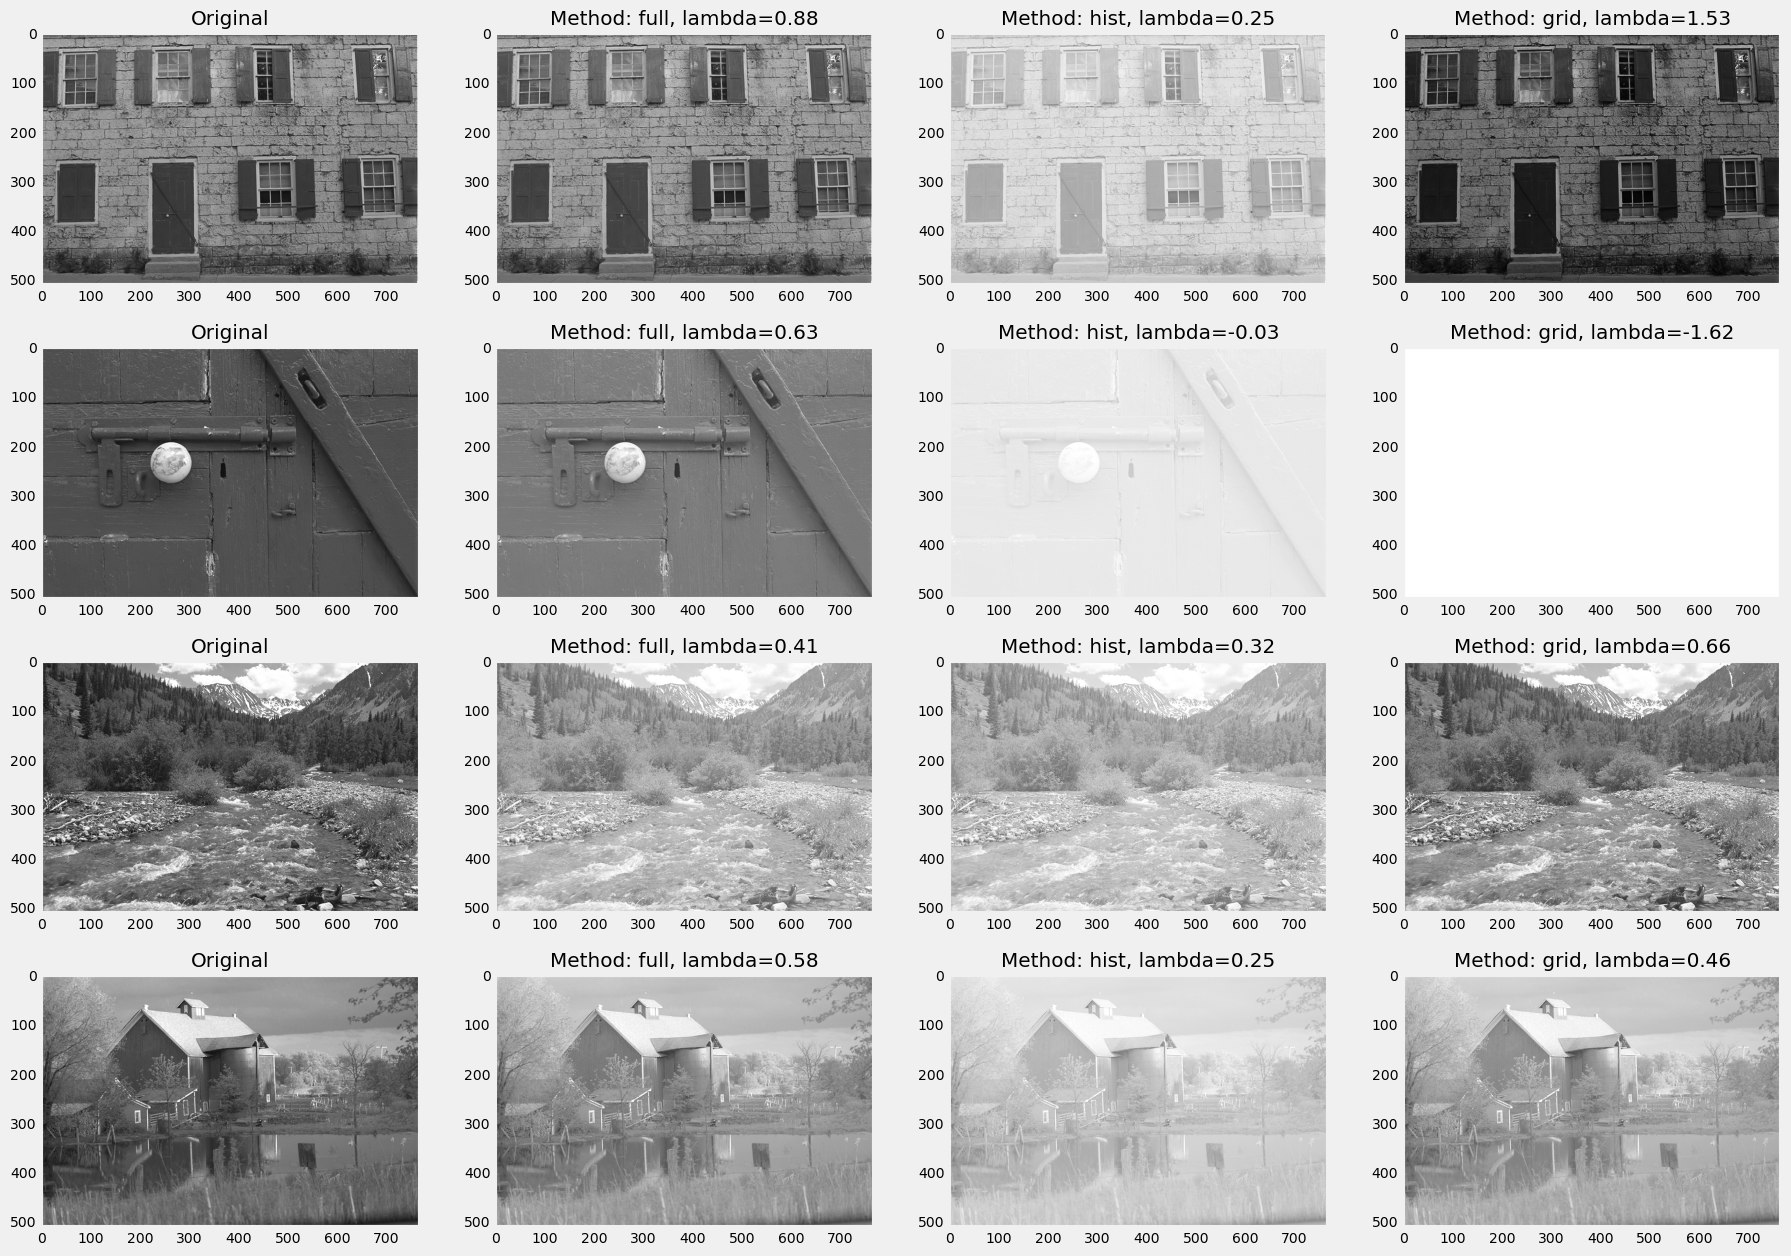
\includegraphics[width=0.7\textwidth]{img_bci_all.png}
        \caption{Transformaciones de la imagen 1, 2, 13, y 22. De izquierda a derecha, imagen original, m\'etodo de datos completos, m\'etodo de histograma, y m\'etodo de grilla.}
        \label{fig:img_bci_all}
    \end{figure}
\end{frame}

\begin{frame}{La transformación Box-Cox}
    \begin{center}
        {\Large ¿Qué valores de $\lambda$ obtenemos?}
    \end{center}
\end{frame}


\begin{frame}{La transformación Box-Cox}
    \begin{figure}[H]
        \centering
        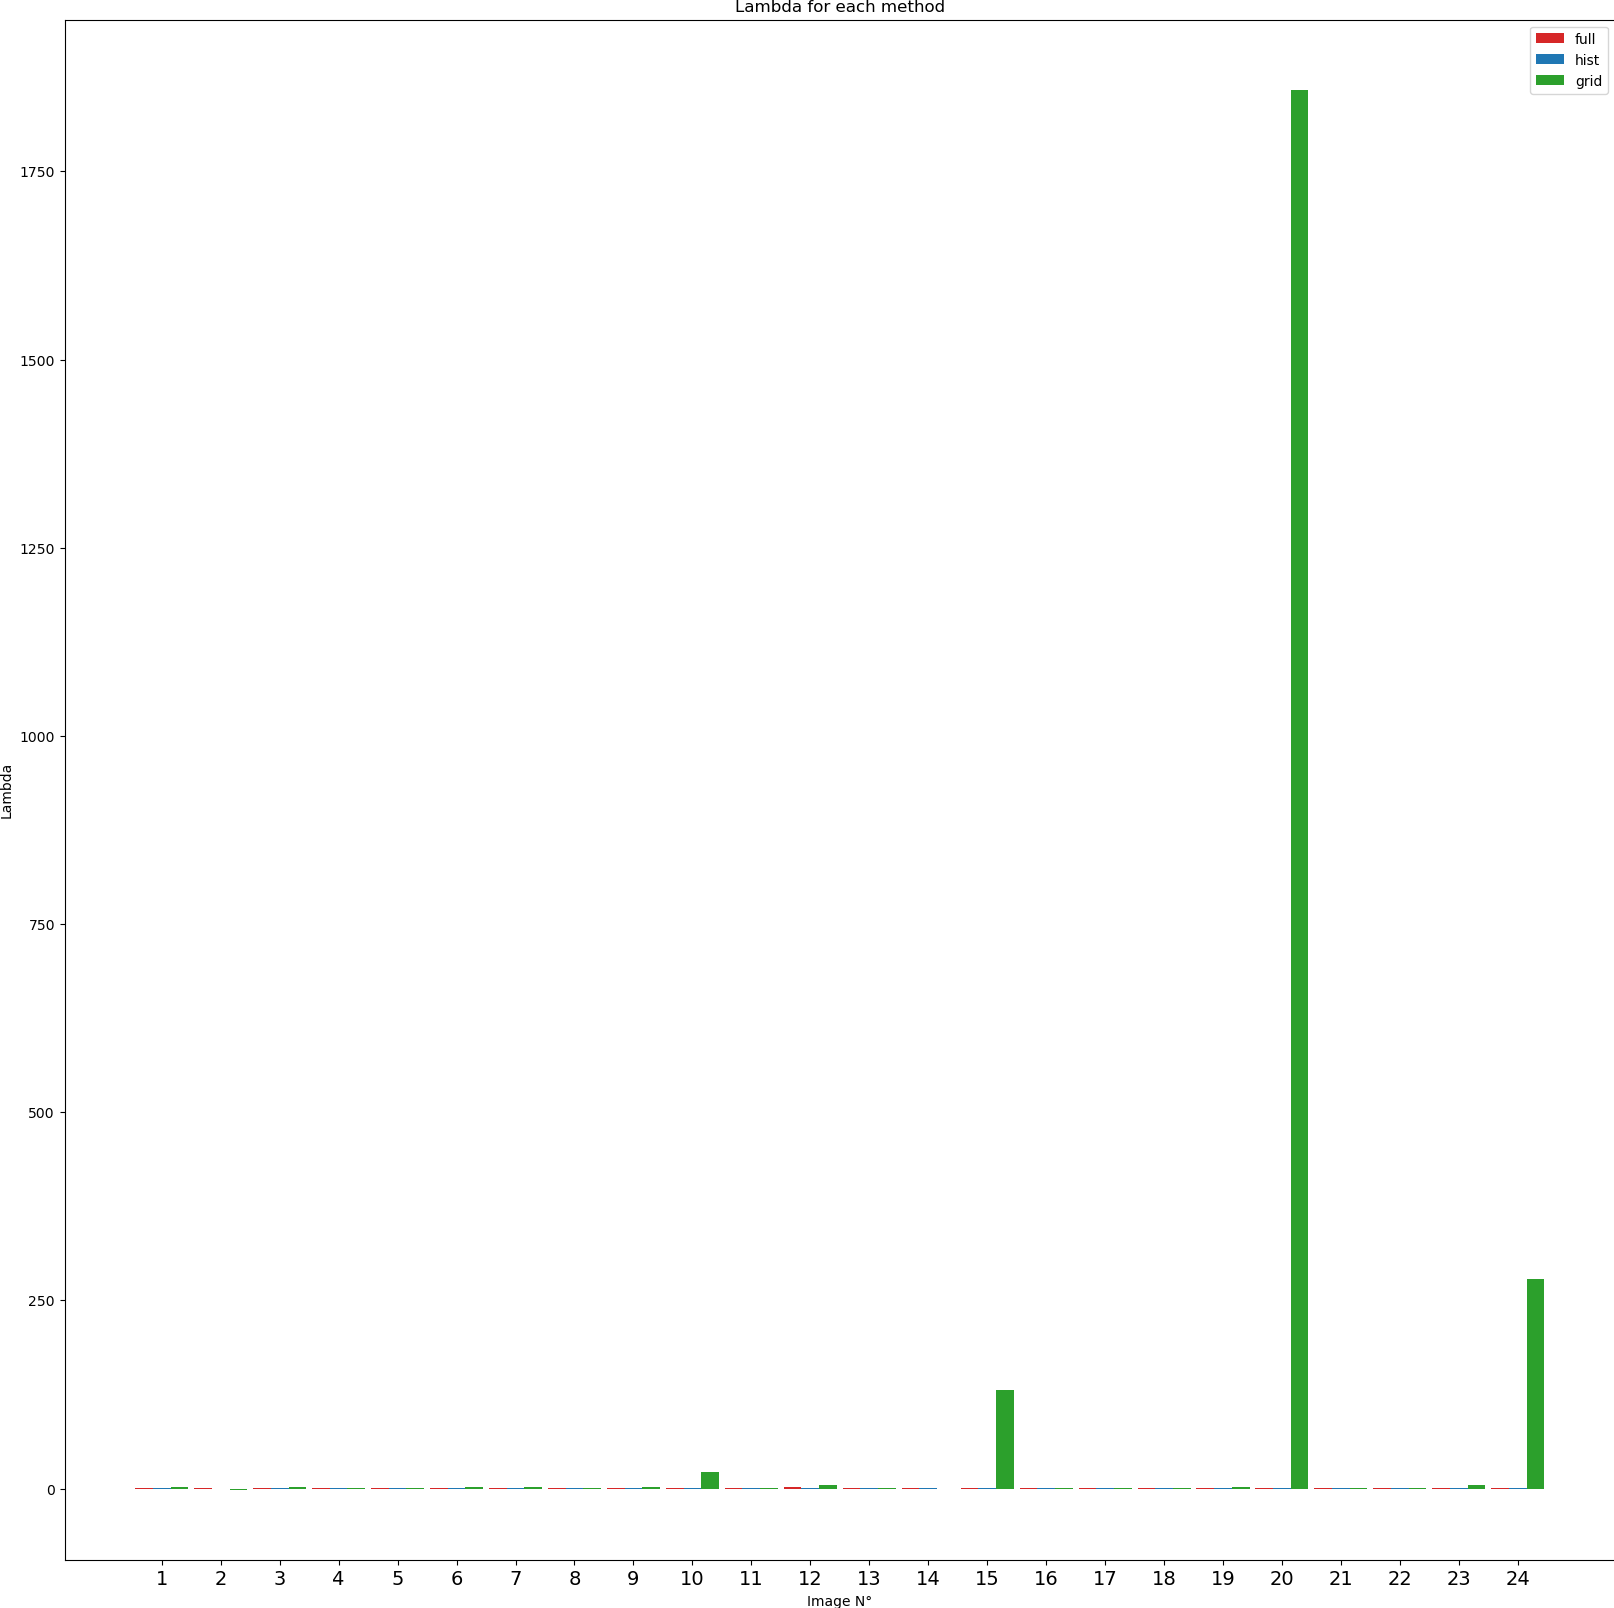
\includegraphics[width=0.5\textwidth]{lambda_noclip.png}
        \caption{Valores de $\lambda$ para todo el banco de imagenes. verde es el m\'etodo de grilla, azul es el m\'etodo de histograma, y rojo es el m\'etodo de datos completos.}
        \label{fig:lambda_noclip}
    \end{figure}
\end{frame}

\begin{frame}{La transformación Box-Cox}
    \begin{figure}[H]
        \centering
        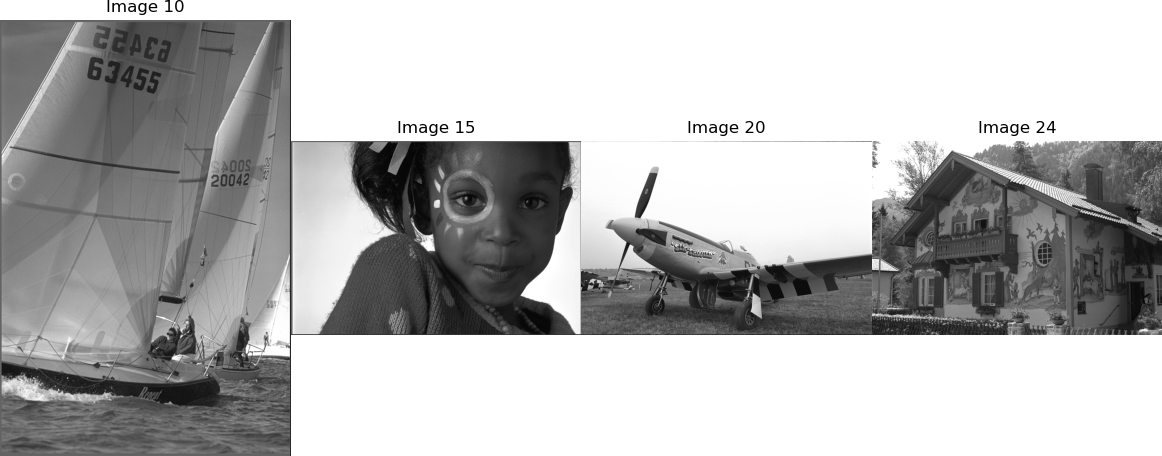
\includegraphics[width=0.9\textwidth]{img_ex_10_15_20_24.png}
        \caption{Transformaciones de las imagenes 10, 15, 20, y 24.}
        \label{fig:img_bci_10_15_20}
    \end{figure}
\end{frame}

\begin{frame}{La transformación Box-Cox}
    \begin{figure}[H]
        \centering
        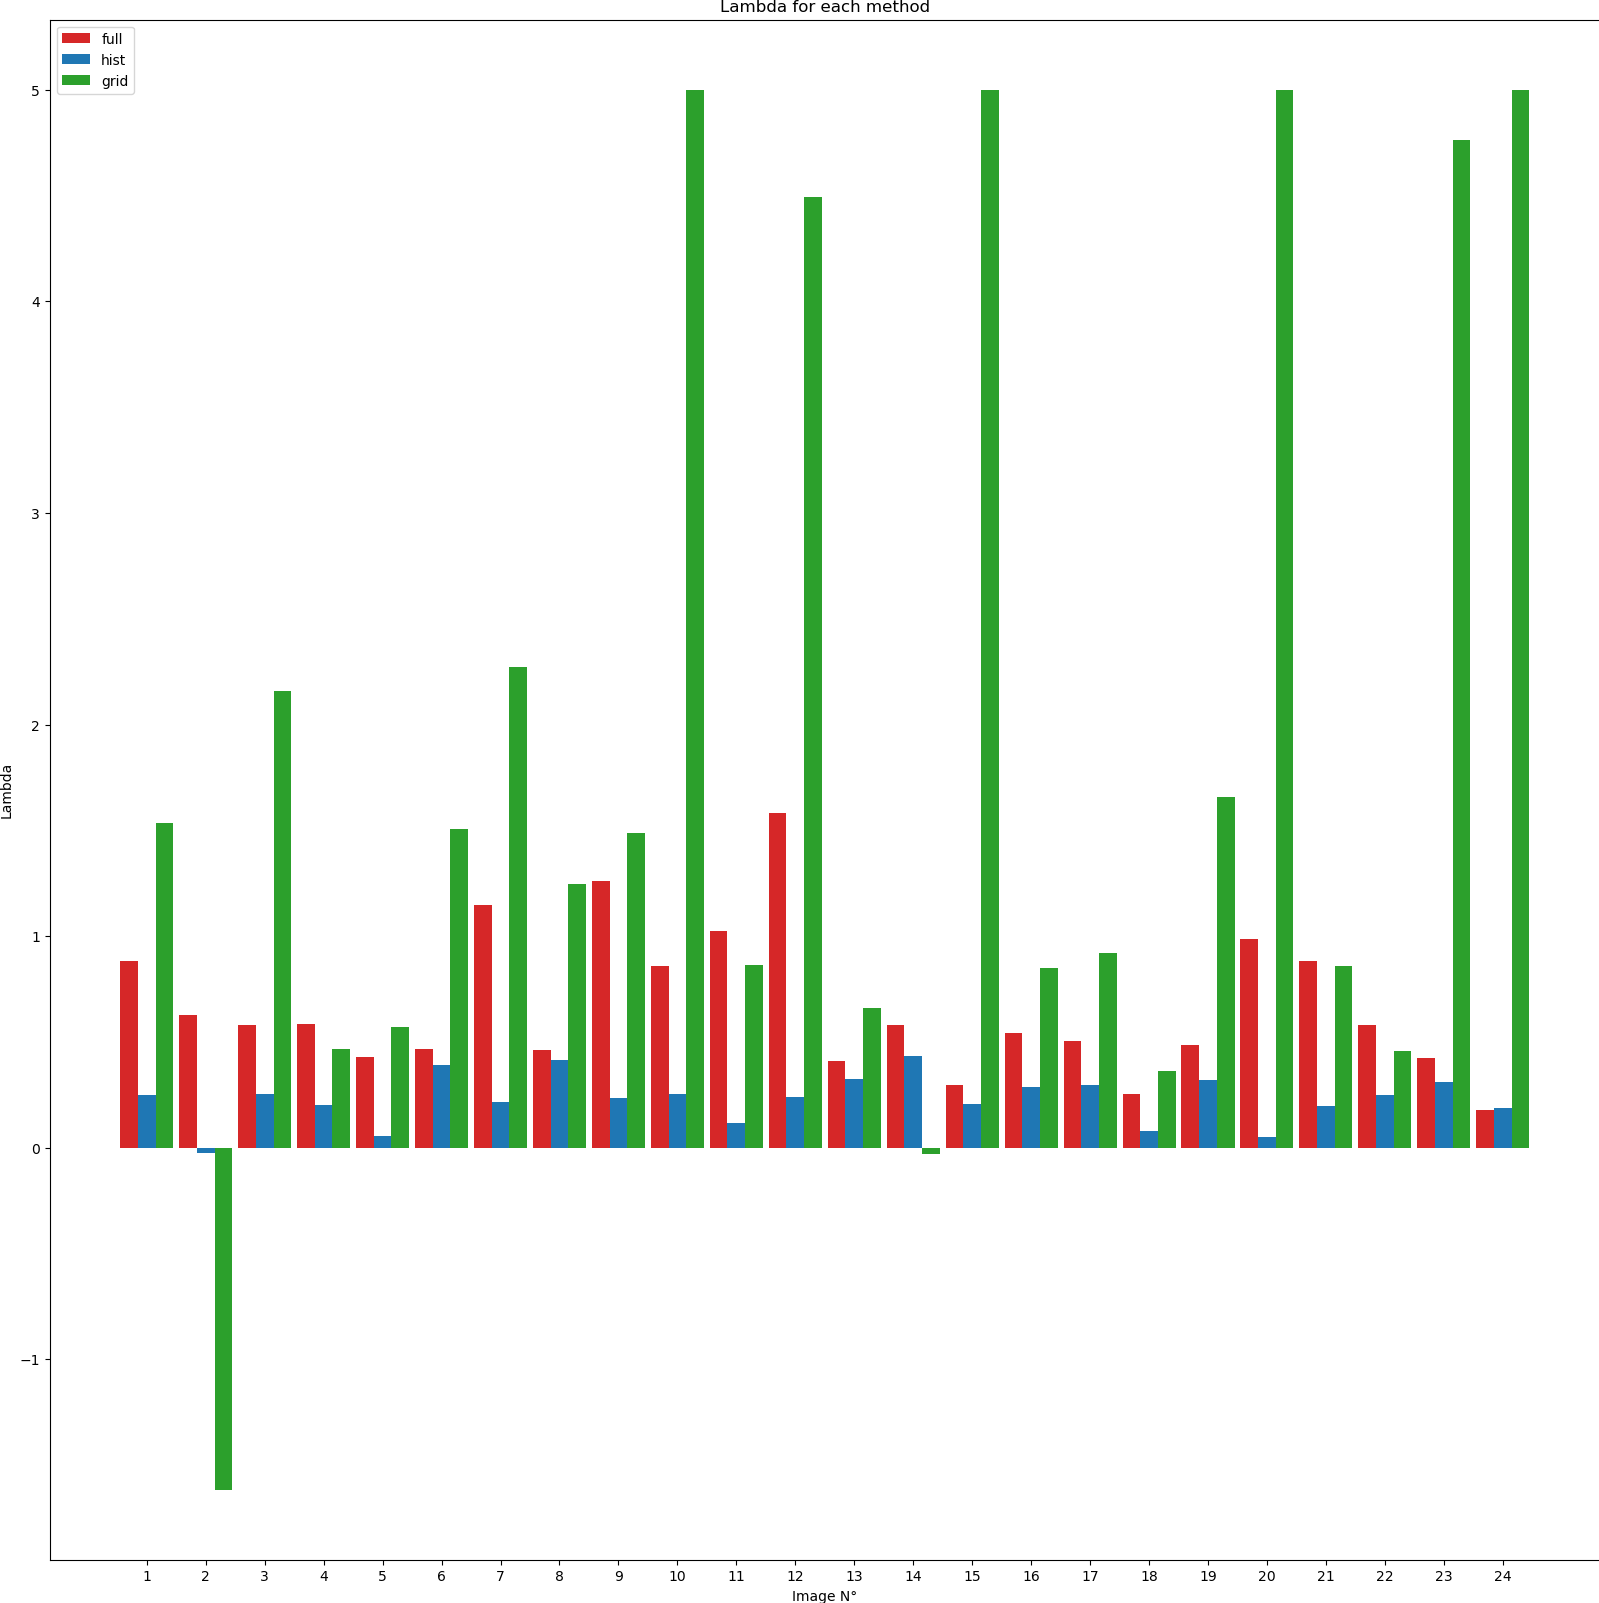
\includegraphics[width=0.5\textwidth]{lambda_clip.png}
        \caption{Valores de $\lambda$ para todo el banco de imagenes, cortado en 5. verde es el m\'etodo de grilla, azul es histograma, y rojo es datos completos}
        \label{fig:lambda_clip}
    \end{figure}
\end{frame}


\begin{frame}{La transformación Box-Cox}
    ¿Cómo se relacionan los valores de $\lambda$ obtenidos por los diferentes métodos? 
    \pause
    \begin{block}{Correlaciones}
        \begin{table}[H]
            \centering
            \begin{tabular}{|l|l|l|l|}
                \hline
                M\'etodo 1 & M\'etodo 2 & Pearson $\rho$ & Valor P \\ \hline
                Completo                  & Histograma                & -0.1305   & 0.5431  \\ 
                Completo                  & Grilla                    & 0.1384    & 0.5191  \\ 
                Histograma                & Grilla                    & -0.3467   & 0.0968  \\ \hline
            \end{tabular}
        \end{table}
    \end{block}
    \pause
    Notemos que Cheddad et al. (2010), encontró una correlación entre el método completo y el del histograma es de $-0.3022$.
\end{frame}



\section{Experimentos Numéricos}
\begin{frame}
    \begin{center}
        {\LARGE\bf Experimentos Numéricos}
    \end{center}
\end{frame}


\begin{frame}{Experimentos Numéricos}
    \pause
    Para estos experimentos utilizamos el banco de imágenes mostrado anteriormente. Para cada imagen, hacemos la transformación para un rango de valores, además de los valores de $\lambda$ obtenidos por los métodos de grilla, histograma, y completo.
    
    \begin{figure}[H]
        \centering
        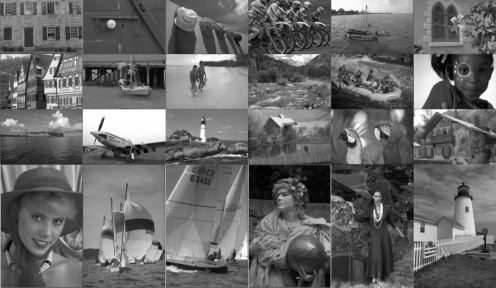
\includegraphics[width=0.4\textwidth]{all_images_grid_bw.png}
    \end{figure}
    \pause
    Luego,utilizaremos los métodos de correlación de MIC y dCor; comparando el vector completo y el histograma de las imágenes transformadas con la imagen original.
    
    Además se muestra la correlación de Pearson $\rho$ como base de comparación.
\end{frame}

\begin{frame}{Experimentos Numéricos}
    \begin{center}
        {\Large\bf Rango de valores para $\lambda$}
    \end{center}
    \pause

    \begin{center}
        {\Large  Comparando los vectores de las imágenes.}
    \end{center}
\end{frame}


\begin{frame}{Experimentos Numéricos}
    
    \begin{figure}[H]
        \centering
        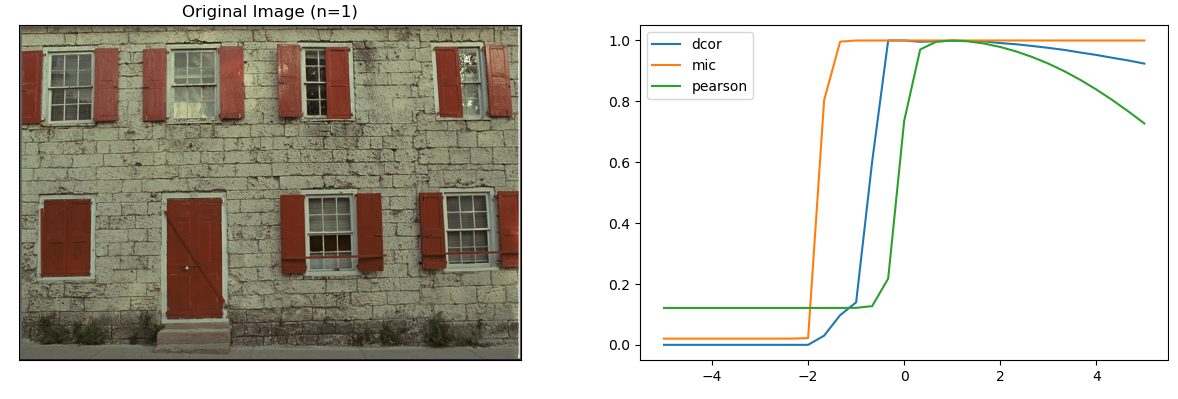
\includegraphics[width=\textwidth]{lam_v_com_one.png}
        \caption{De arriba hacia abajo, imagen 1. A la izquierda la imagen original y a la derecha el valor de $dCor$ (azul), $MIC$ (naranja), y $\rho$ (verde) en el eje y, $\lambda$ en el eje x.}
    \end{figure}
\end{frame}

\begin{frame}{Experimentos Numéricos}
    Comparando los vectores de las imágenes.
    \begin{figure}[H]
        \centering
        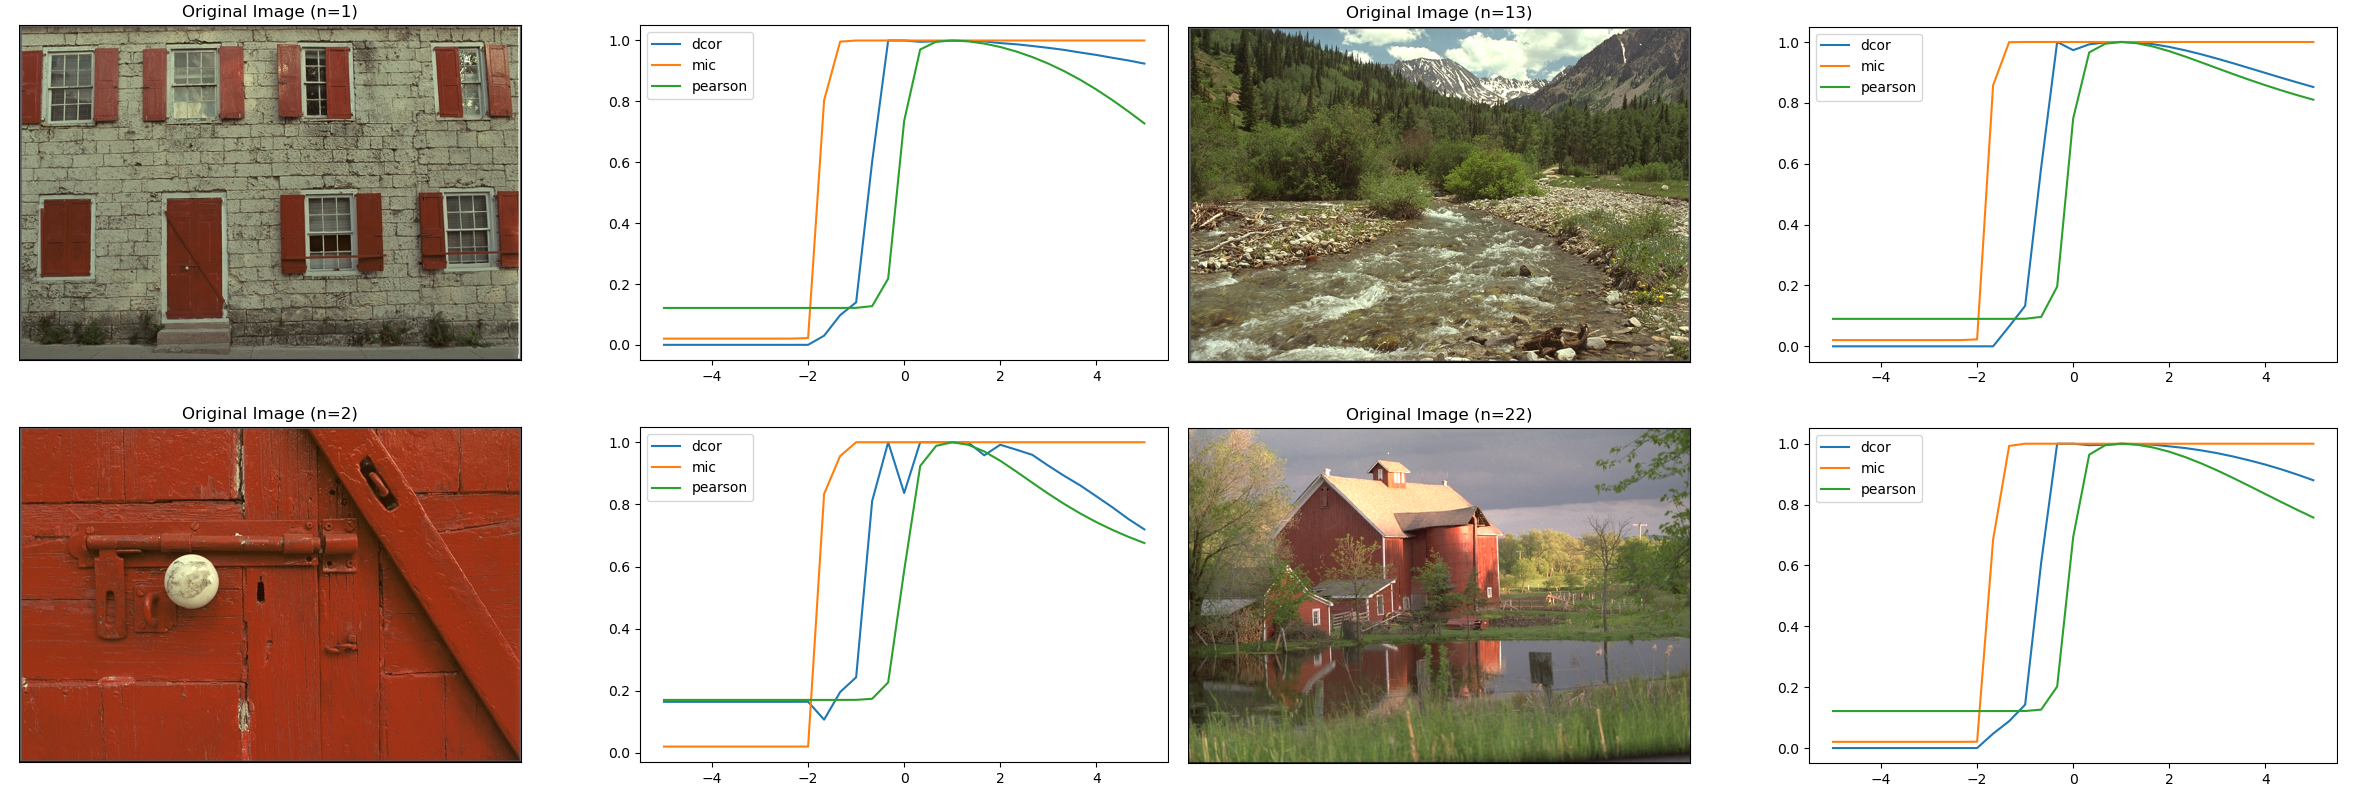
\includegraphics[width=\textwidth]{lam_v_com_all_img.png}
        \caption{De arriba hacia abajo, imagenes 1, 2, 13, y 22. A la izquierda la imagen original y a la derecha el valor de $dCor$ (azul), $MIC$ (naranja), y $\rho$ (verde) en el eje y, $\lambda$ en el eje x.}
    \end{figure}
\end{frame}


\begin{frame}{Experimentos Numéricos}
    \begin{center}
        {\Large\bf Rango de valores para $\lambda$}
    \end{center}
    \pause

    \begin{center}
        {\Large  Comparando el histograma de las imágenes.}
    \end{center}
\end{frame}
\begin{frame}{Experimentos Numéricos}
    \begin{figure}[H]
        \centering
        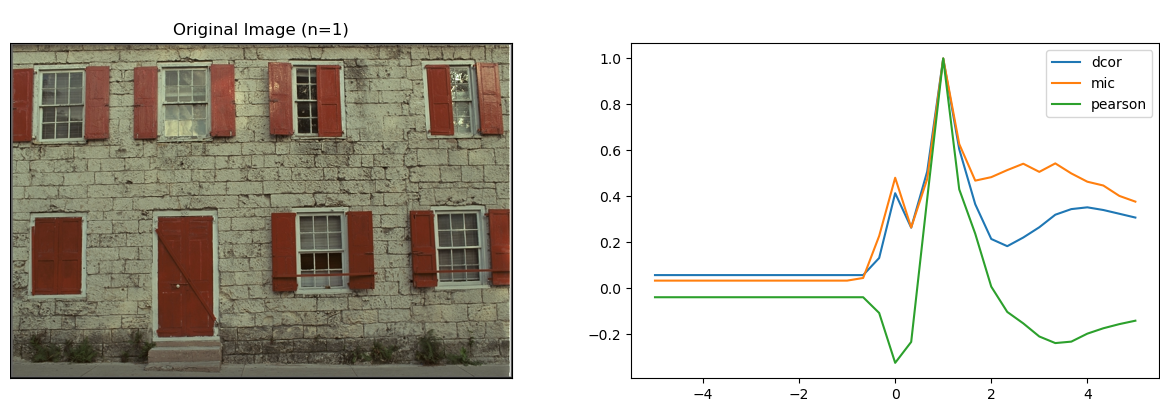
\includegraphics[width=\textwidth]{lam_v_com_one_hist.png}
        \caption{De arriba hacia abajo, imagenes 1, 2, 13, y 22. A la izquierda la imagen original y a la derecha el valor de $dCor$ (azul), $MIC$ (naranja), y $\rho$ (verde) en el eje y, $\lambda$ en el eje x.}
    \end{figure}
\end{frame}

\begin{frame}{Experimentos Numéricos}
    \begin{figure}[H]
        \centering
        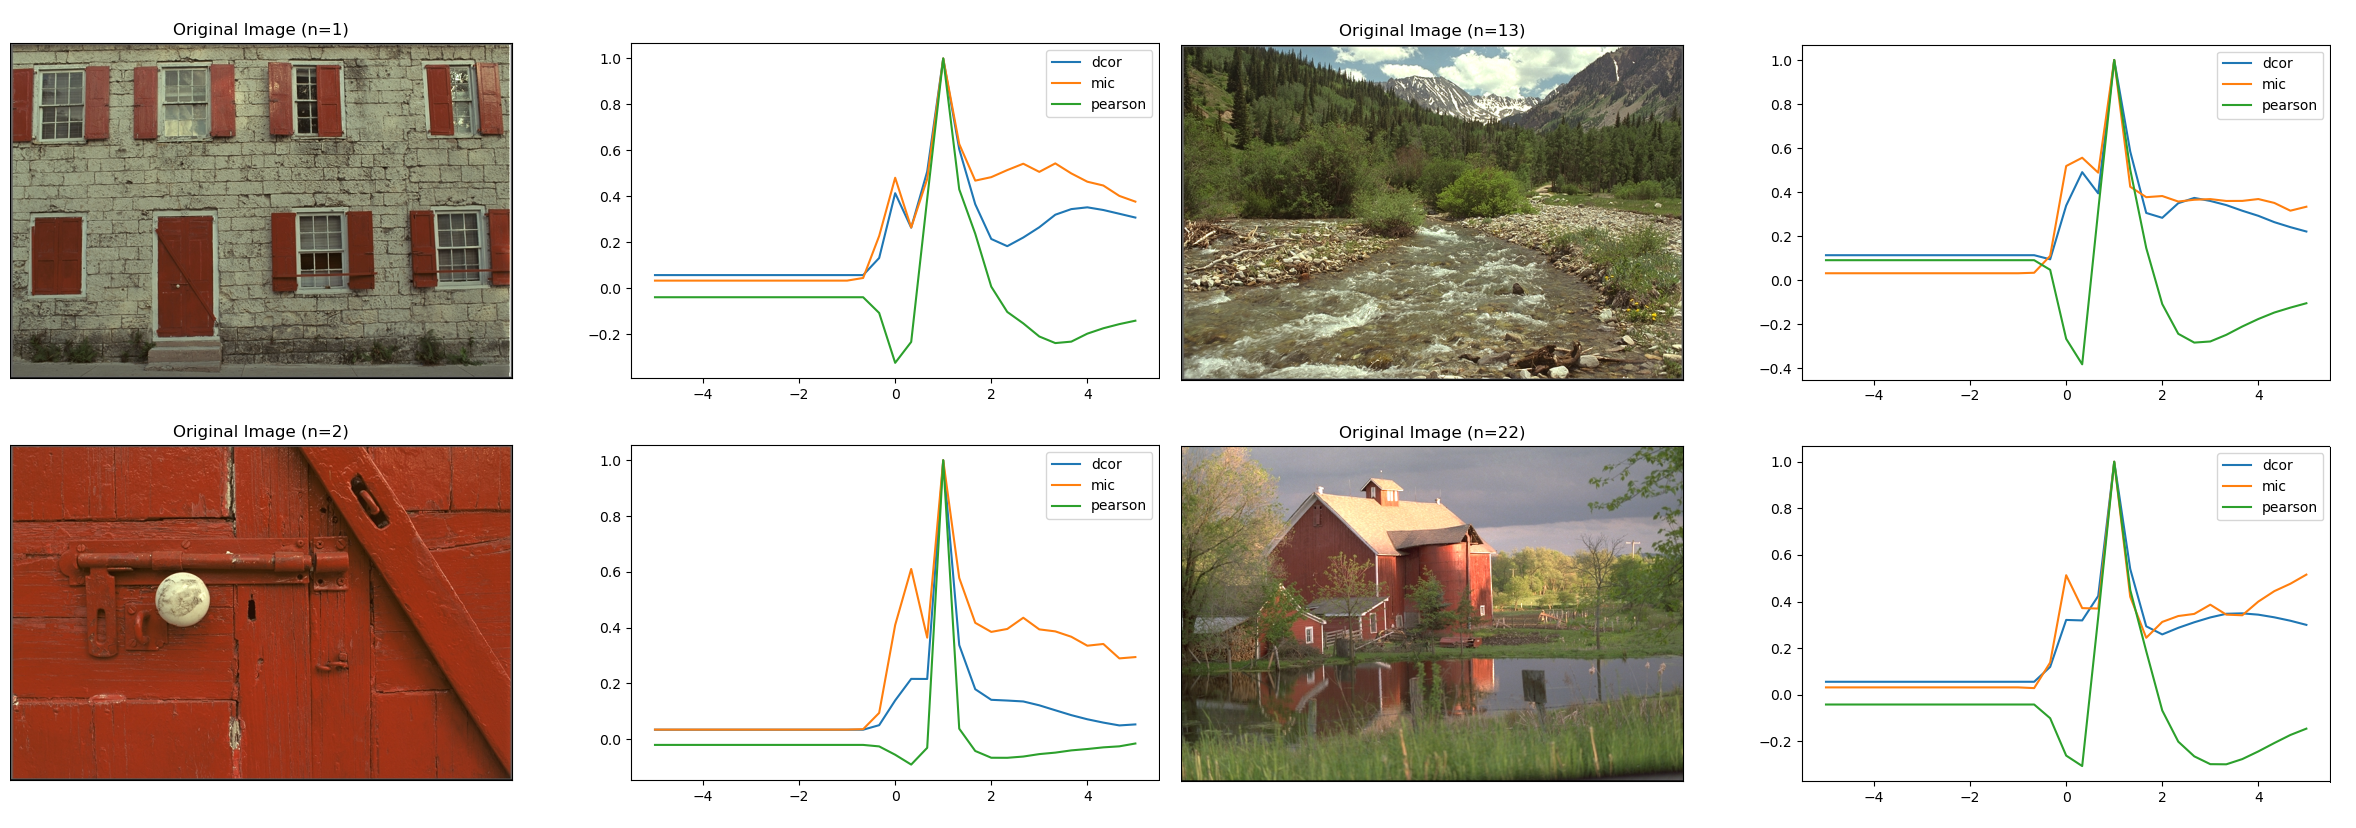
\includegraphics[width=0.8\textwidth]{lam_v_com_all_img_hist.png}
        \caption{De arriba hacia abajo, imagenes 1, 2, 13, y 22. A la izquierda la imagen original y a la derecha el valor de $dCor$ (azul), $MIC$ (naranja), y $\rho$ (verde) en el eje y, $\lambda$ en el eje x.}
    \end{figure}
\end{frame}

\begin{frame}{Experimentos Numéricos}
    \begin{center}
        {\Large\bf Valores seleccionados de $\lambda$}
    \end{center}
    \pause

    \begin{center}
        {\Large  Comparando los vectores de las imágenes.}
    \end{center}
\end{frame}

\begin{frame}{Experimentos Numéricos}
    \begin{figure}[H]
        \centering
        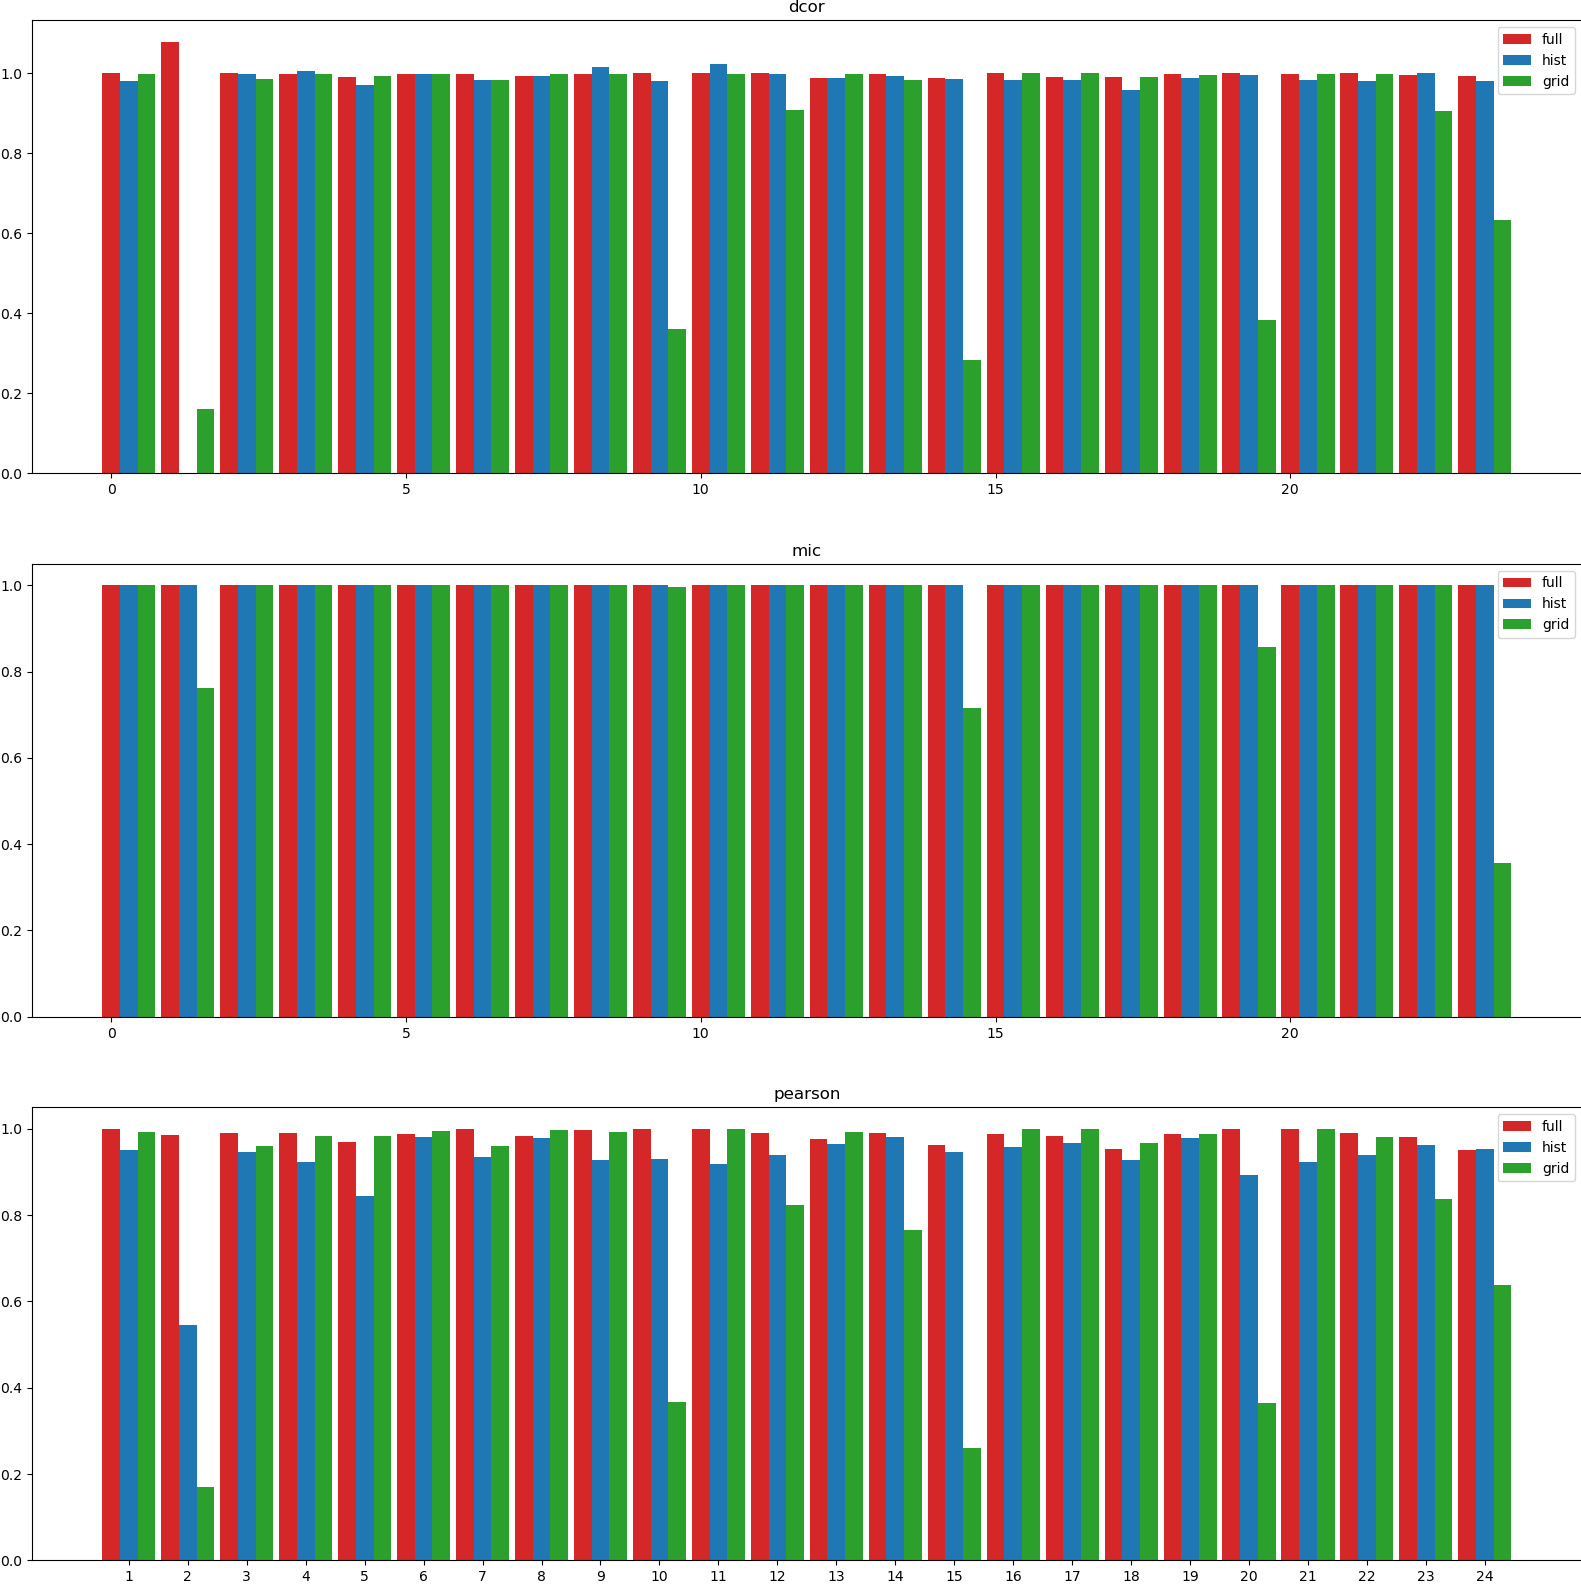
\includegraphics[width=0.55\textwidth]{plot_comparison_full.png}
        \caption{Valores de dcor, mic y pearson para cada imagen usando todo el vector, azul es el metodo para encontrar $\lambda$ con toda la imagen, rojo es el histograma y verde es el grilla.}
    \end{figure}
\end{frame}

\begin{frame}{Experimentos Numéricos}
    \begin{figure}[H]
        \centering
        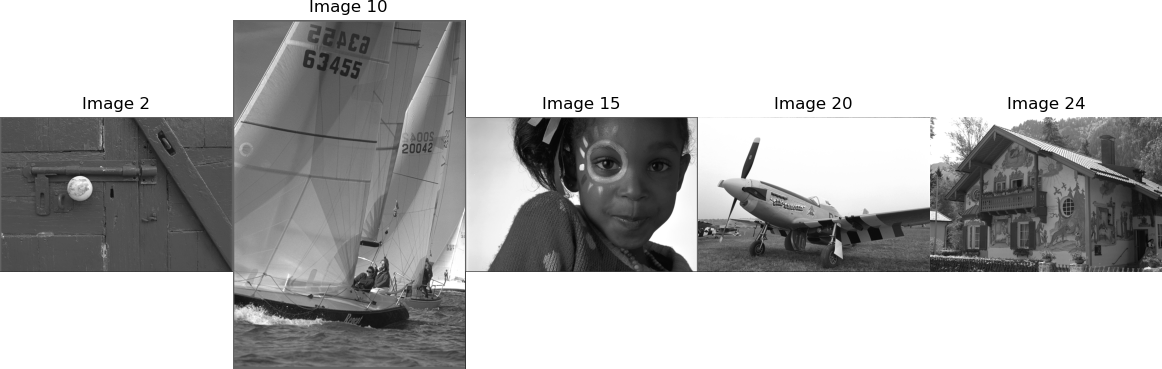
\includegraphics[width=\textwidth]{anomalies_grid.png}
    \end{figure}
    De izquierda a derecha, imagenes 2, 10, 15, 20, y 24 del banco.Estos corresponden a los valores an\'omalos en el m\'etodo de grilla.
\end{frame}



\begin{frame}{Experimentos Numéricos}
    Los promedio de los valores de correlación para cada método, comparando los vectores de las imágenes son:
    \pause
    \begin{block}{Corr.} 
        \begin{table}[H]
            \centering
            \begin{tabular}{|l|l|l|}
                \hline
            Correlaci\'on    & $\lambda$ & Valor  \\    \hline
            dcor    & Completo    & 1.000  \\
            mic     & Completo    & 1.000  \\
            mic     & Histograma  & 1.000  \\
            pearson & Completo    & 0.985 \\
            dcor    & Histograma  & 0.948 \\
            mic     & Grilla      & 0.945  \\
            pearson & Histograma  & 0.925  \\
            dcor    & Grilla      & 0.945  \\
            pearson & Grilla      & 0.856  \\     \hline
            \end{tabular}
        \end{table}
    \end{block}
\end{frame}
\begin{frame}{Experimentos Numéricos}
    \begin{center}
        {\LARGE\bf Valores seleccionados de $\lambda$}
    \end{center}
    \pause
    \begin{center}
        {\Large  Comparando el histograms de las imágenes. $\lambda$}
    \end{center}
\end{frame}

\begin{frame}{Experimentos Numéricos}
    \begin{figure}[H]
        \centering
        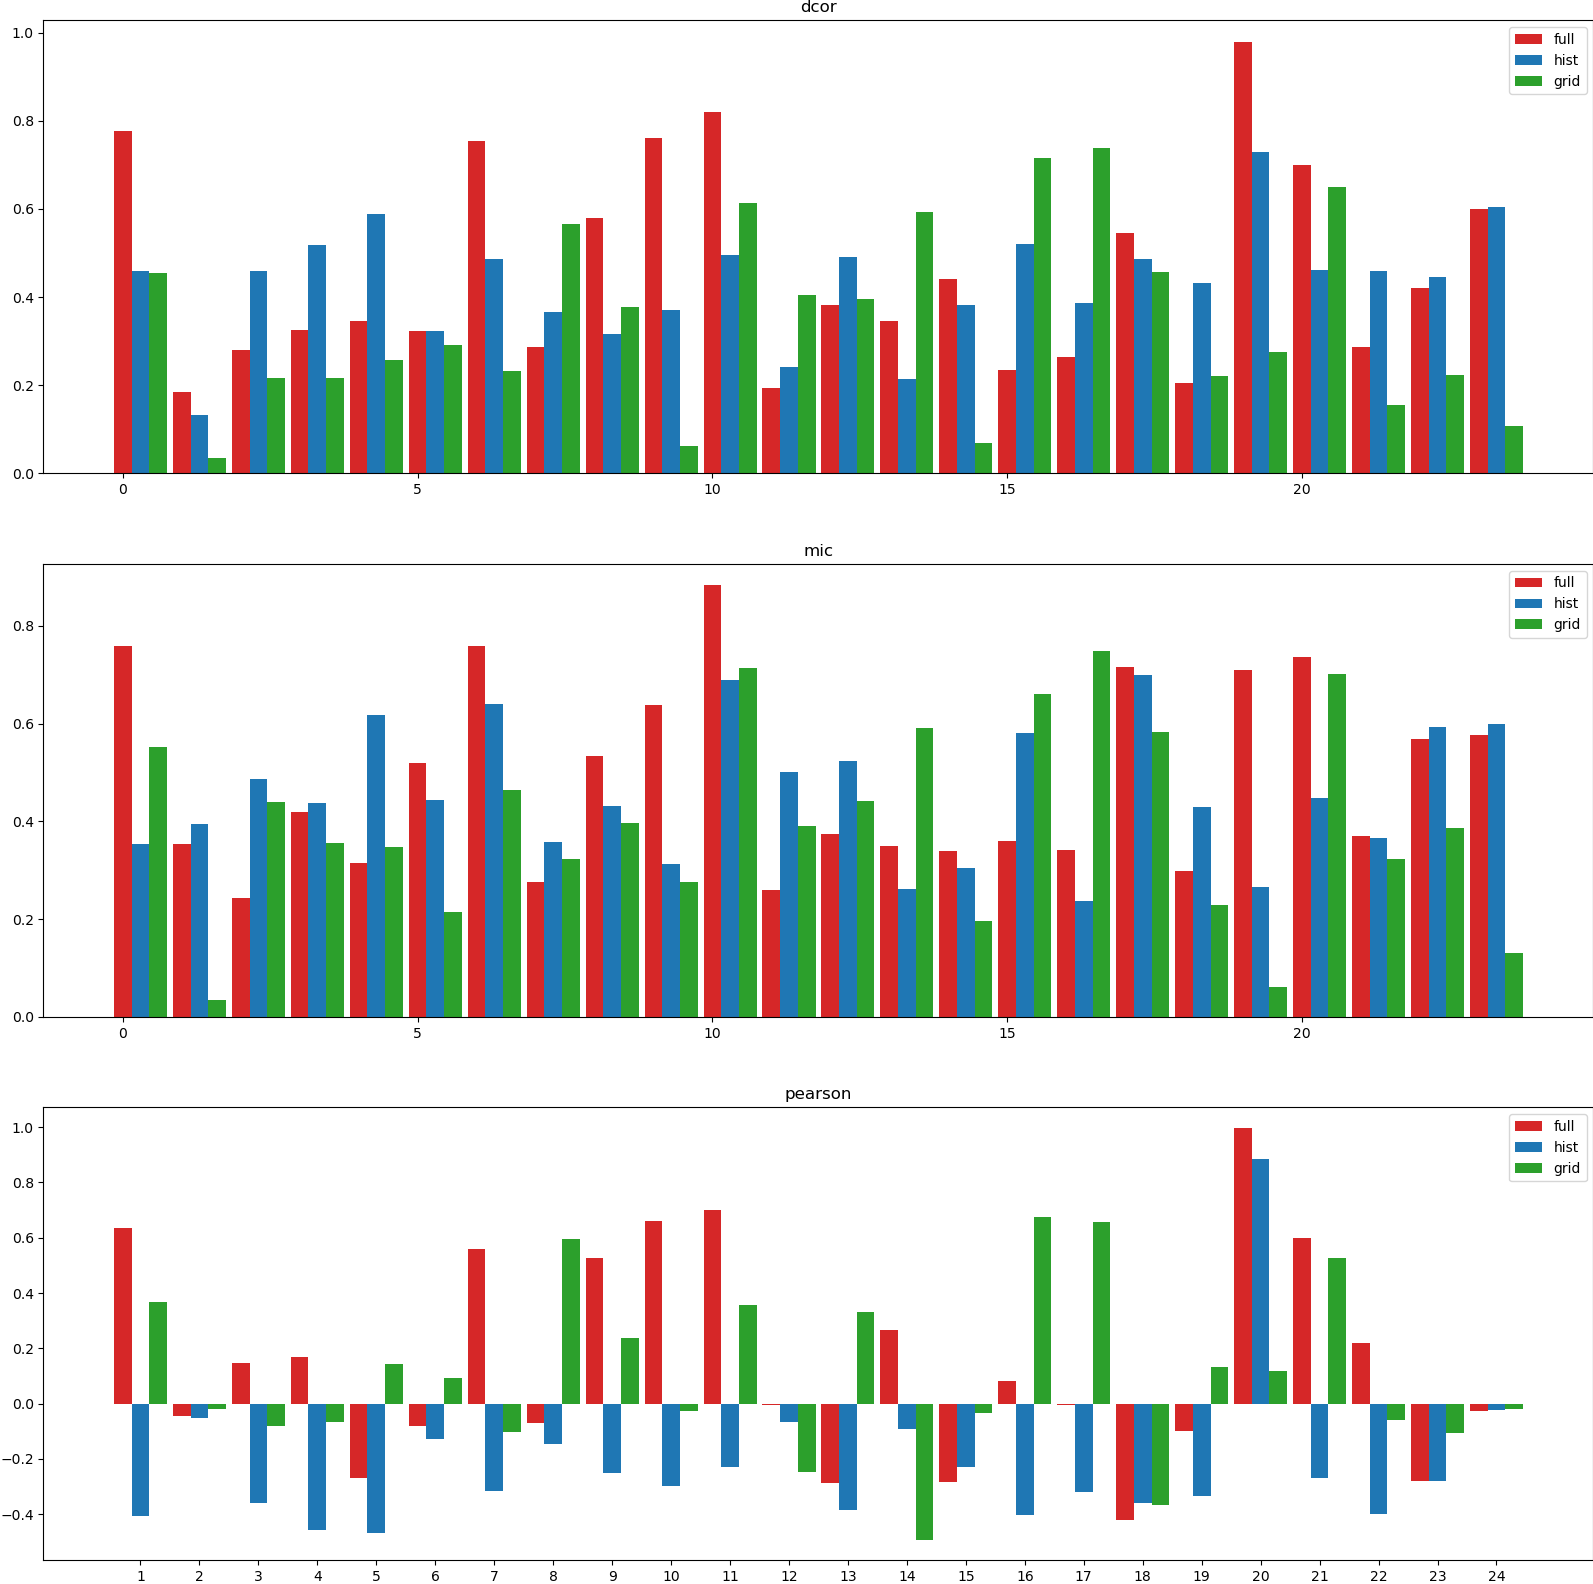
\includegraphics[width=0.6\textwidth]{plot_comparison_hist.png}
        \caption{Valores de dcor, mic y pearson para cada imagen usando el histograma, azul es el metodo para encontrar $\lambda$ con toda la imagen, rojo es el histograma y verde es el grid}
    \end{figure}
\end{frame}

\begin{frame}{Experimentos Numéricos}
    El promedio de los valores de correlación para cada método comparando el histograma de las imágenes son:
    \pause
    \begin{block}{Corr.} 
        \begin{table}[H]
            \centering
            \begin{tabular}{|l|l|l|}\hline
            Correlaci\'on    & $\lambda$ & Valor  \\    \hline
            mic     & Completo    & 0.487  \\
            dcor    & Completo    & 0.459  \\
            mic     & Histograma  & 0.457  \\
            dcor    & Histograma  & 0.431  \\
            mic     & Grilla      & 0.398  \\
            dcor    & Grilla      & 0.346 \\
            pearson & Completo    & 0.108  \\
            pearson & Grilla      & 0.108  \\
            pearson & Histograma  & -0.225 \\\hline
            \end{tabular}
        \end{table}
    \end{block}
\end{frame}

\section{Conclusiones}

\begin{frame}{Conclusiones}
    
    \begin{itemize}
        \pause
        \item Dentro de un rango para $\lambda$, las imágenes transformadas con Box-Cox están fuertemente corelacionadas con sus primitivas. 
        \pause
        \item Los métodos de estudiados para la selección de $\lambda$ son útiles para encontrar valores que maximizan la correlación entre las imágenes, a excepción del método de grilla, que puede ser \textit{instable}.
        \pause
        \item La transformación de Box-Cox puede ser útil normalizar imágenes. Las imágenes transformadas mantienen una alta correlación con las imágenes originales.
        \pause
        \item La comparación entre imágenes es compleja, y no hay un método claro o único para hacerlo.
    \end{itemize}
\end{frame}

\begin{frame}{Trabajos Futuros}
    \begin{itemize}
        \pause
        \item Explorar otros métodos de selección de $\lambda$.
        \pause 
        En particular, algunos que no involucren a la Verosimilitud.
        \pause 
        \item Explorar trabajar $\lambda$ como una función $\lambda(x, y)$.
        \pause
        \item Explorar otros métodos de comparación de imágenes.
    \end{itemize}
    
\end{frame}


\begin{frame}{Bibliografía}
    \begin{thebibliography}{9}
    \bibitem{boxcox}
    Box, G. and Cox, D., 1964. An Analysis of Transformations. Journal of the Royal Statistical Society, 26(2).
    
    \bibitem{Szekely2009}
    Székely, G. J., Rizzo, M. L. and Bakirov, N. K. (2007). Measuring and testing independence by correlation of distances. Ann. Statist.

    \bibitem{reshef2011}
    Reshef, D., Reshef, Y., Finucane, H., Grossman, S., McVean, G., Turnbaugh, P., Lander, E., Mitzenmacher, M. and Sabeti, P., 2011. Detecting Novel Associations in Large Data Sets. Science.
    \bibitem[]{cheddad2020}
    Cheddad, A., 2020. On Box-Cox Transformation for Image Normality and Pattern Classification. IEEE Access.
    
    \bibitem[]{juin2009}
    Juin-Der Lee, Hong-Ren Su, Cheng, P., Liou, M., Aston, J., Tsai, A. and Cheng-Yu Chen, 2009. MR Image Segmentation Using a Power Transformation Approach. IEEE Transactions on Medical Imaging.
    \end{thebibliography}
\end{frame}
\end{document}




